\documentclass[12pt,a4paper]{article}

% ---------- Language & typography ----------
\usepackage[T1]{fontenc}
\usepackage[utf8]{inputenc}
\usepackage[numbers]{natbib} % <--- Natbib AVANT babel comme demandé !
\usepackage[french]{babel}
\usepackage{lmodern}
\usepackage{amsmath}
\usepackage{amssymb}
\usepackage{xcolor} 
\usepackage[normalem]{ulem} 
\usepackage{subcaption}

% ---------- Nouveaux packages pour régler tes erreurs ----------
\usepackage{float}    % Pour utiliser [H] dans les figures/tables
\usepackage{booktabs} % Pour utiliser \toprule, \midrule, \bottomrule

% ---------- Layout ----------
\usepackage{geometry}
\geometry{margin=2.5cm}
\usepackage{setspace}
\onehalfspacing
\usepackage{parskip} 

% ---------- Graphics & links ----------
\usepackage{graphicx}
\usepackage[hidelinks]{hyperref}
\begin{document}

% =======================
% Page de garde (identique à ton rapport)
% =======================
\begin{titlepage}
  \thispagestyle{empty}
  \centering

  \noindent
  \begin{minipage}[t]{0.49\textwidth}
    
\includegraphics[height=2cm]{Logo-ENPC-IP-RVB.png}
  \end{minipage}
  \hfill
  \begin{minipage}[t]{0.49\textwidth}
    \raggedleft
    
\includegraphics[height=2cm]{cermics.jpeg}
  \end{minipage}

  {\Large \textsc{École Nationale des Ponts et Chaussées}\par}
  \vspace{1.0cm}

  {\large \textbf{PROJET DE PREMIÈRE ANNÉE 2026}\par}
  {\large \textbf{RAPPORT FINAL}\par}
  \vspace{1.5cm}

  {\LARGE \textbf{Réduction de modèle : Proper Orthogonal Decomposition (POD)
et méthode des bases réduites}\par}
  \vspace{1.6cm}

  {\large \textbf{Yasmine EL HOUARI, Antonin AYE, Mathis BORIE, Marek PIOT}\par}
  \vspace{1.2cm}

  {\large sous la direction de\par}
  \vspace{0.4cm}

  {\large \textbf{Sofiane EZZEHI}\par}
  {\large CERMICS\par}

  \vfill
\end{titlepage}

% =======================
% Table des matières
% =======================
\tableofcontents
\newpage

% =======================
% Main content
% =======================

\section{Problématique générale et modélisation}

\subsection{Problème physique : Les fluides et les écoulements de Darcy}

En physique, un fluide sous pression traversant un milieu poreux cherche toujours 
à minimiser son énergie. Tout comme une bille dévale une pente pour atteindre le 
point le plus bas, un fluide va naturellement s'écouler en empruntant le chemin de moindre 
résistance pour dissiper le moins d'énergie possible.

Le fluide se déplace sous l'effet d'un gradient de pression $\nabla u$, où $u$ désigne la pression. 
Cependant, le fluide ne s'écoule pas dans le vide : il frotte contre les parois du milieu. La vitesse d'écoulement du fluide, notée $\mathbf{v}$, est dictée par la loi empirique de Darcy \cite{darcy_wiki} : 
$\mathbf{v} = -D \nabla u$, où $D$ est un coefficient empirique qui dépend du fluide et du milieu.

L'énergie volumique dissipée localement par ce frottement visqueux correspond au travail de cette vitesse contre le gradient de pression, valant ainsi $\frac{1}{2} D \nabla u \cdot \nabla u$. 
En opposition à cette perte d'énergie, on peut considérer le travail fourni au système 
par une source externe de fluide (comme un puits d'injection ou de pompage), modélisée 
par un terme $f$.

Le principe de minimisation de l'énergie revient alors à chercher le champ de pression $u$ 
qui minimise la fonctionnelle $J(u)$ totale sur le domaine étudié $\Omega$ :
\begin{equation*}
    J(u) = \int_{\Omega} \frac{1}{2} D \nabla u \cdot \nabla u \, d\Omega - \int_{\Omega} f u \, d\Omega,
\end{equation*}
La condition du premier ordre pour minimiser cette énergie impose que sa dérivée s'annule. En appliquant une intégration par parties à cette condition, le problème se sépare mathématiquement en deux composantes. Pour que l'équilibre soit garanti, le fluide doit vérifier une équation différentielle locale à l'intérieur du domaine $\Omega$, et simultanément respecter les contraintes imposées sur les bords $\partial \Omega$ (par exemple, une pression imposée $\bar{u}$, appelée condition de Dirichlet). On obtient ainsi le système complet \cite{darcy_wiki} :
\begin{equation}
  \label{probleme Darcy}
    \begin{cases}
        -\nabla \cdot (D \nabla u) = f & \text{dans } \Omega \\
        u = \bar{u} & \text{sur } \partial \Omega
    \end{cases}
\end{equation}

\subsection{Les paramètres du projet}

Le problème de Darcy étudié dans ce projet se place dans un contexte d'écoulement en milieu poreux fracturé. Le domaine d'étude $\Omega$ est le carré unité $[0,1]^2$, discrétisé par un maillage régulier de $200 \times 200$ éléments triangulaires, produisant $N_{\text{dof}} = 80\,402$ degrés de liberté. Les éléments finis choisis sont des polynômes de degré 2, offrant un bon compromis entre précision et coût de calcul.

\subsubsection{Conditions aux limites}

Les conditions aux limites de Dirichlet imposées aux frontières du domaine $\partial \Omega$ sont :
\begin{equation}
    u_D(x, y) = \begin{cases}
        4.0 & \text{si } (x < 0.1 \text{ et } y > 0.9) \\
        1.0 & \text{si } y < 0.1  \\
        0.0 & \text{ailleurs}
    \end{cases}
\end{equation}
Ces conditions aux limites représentent deux sources de pression (haut-gauche et bas) et un puits en aval, reproduisant un scénario physiquement réaliste d'injection de fluide et de drainage.

\subsubsection{Fonction de conductivité paramétrique}

La conductivité $k(x, y; \mu)$ est le cœur de la paramétrisation du problème. Elle modélise une fracture de géométrie variable dans un milieu homogène. La conductivité du problème est définie comme telle :
\begin{equation}
    k(x, y; \mu) = D_{\text{back}} + (D_{\text{frac}} - D_{\text{back}}) \cdot H(\mathcal{D}(x, y; a, x_0, w))
\end{equation}
où $\mathcal{D}(x, y; a, x_0, w) = -ax - y + x_0 - w$ définit la distance signée à la fracture, et $H(\cdot)$ est une fonction Heaviside.


\subsubsection{Espace des paramètres}

Le vecteur de paramètres $\mu$ est de dimension 5 :
\begin{equation}
    \mu = (a, x_0, w, D_{\text{back}}, D_{\text{frac}}) \in \mu_{\text{ad}} \subset \mathbb{R}^5
\end{equation}

Les plages autorisées sont :
\begin{align}
    a &\in [20, 60] \quad \text{(pente de la fracture en degré)} \\
    x_0 &\in [50, 90] \quad \text{(position verticale)} \\
    w &\in [3, 7] \quad \text{(demi-largeur)} \\
    D_{\text{back}} &\in [80, 120] \quad \text{(conductivité du milieu)} \\
    D_{\text{frac}} &\in [0.5, 2.0] \quad \text{(conductivité de la fracture)}
\end{align}

La dépendance en $(a, x_0, w)$ est \textit{non-linéaire}, tandis que celle en $(D_{\text{back}}, D_{\text{frac}})$ est \textit{affine}. Cette distinction structure toute l'approche de réduction de modèle.


\subsection{Formulation variationnelle}


Dans la suite du projet, nous allons considérer le problème suivant :

Trouver $u \in H^1(\Omega)$ tel que :
\begin{equation}
  \label{probleme1}
  \begin{cases}
      -\nabla \cdot (D \nabla u) = 0 & \text{dans } \Omega, \\ 
      u = \bar{u} & \text{sur } \partial \Omega.
  \end{cases}
\end{equation}

Pour résoudre ce problème, on utilise une technique de relèvement. Soit $u_L \in H^1(\Omega)$ tel que $u_L|_{\partial \Omega} = \bar{u}$. On peut alors chercher des champs de pression $u_0 \in H_0^1(\Omega)$ tels que $u = u_0 + u_L$ soit solution du problème \eqref{probleme1}. Cela permet de poser la formulation variationnelle suivante :

Trouver $u_0 \in H_0^1(\Omega)$ tel que :
\begin{equation}
    a(u_0, v) = L(v) \quad \forall v \in H_0^1(\Omega)
\end{equation}

où les formes bilinéaire et linéaire sont définies par :
\begin{align}
    a(u_0, v) &= \int_{\Omega} D(x, y; \mu) \nabla u_0 \cdot \nabla v \, d\Omega, \\
    L(v) &= -\int_{\Omega} D(x, y; \mu) \nabla u_L \cdot \nabla v \, d\Omega.
\end{align}



Sous cette forme, le terme de droite $L(v)$ représente l'influence des conditions aux limites imposées sur le système.

La forme bilinéaire $a(\cdot, \cdot)$ est continue et coercive :
\begin{align}
    \text{Continuité:} &\quad |a(u, v)| \leq \|k\|_{\infty} \| u\|_                   {H^1} \| v\|_{H^1} \\
                        &\quad |L(v)| \leq \|k\|_{\infty} \|u_L\|_{H^1}\| v\|_{H^1}  \\
    \text{Coercivité:} &\quad a(u, u) \geq \|k\|_{\min} \| u\|_{H^1}^2
\end{align}
avec $\|k\|_{\min} = \min(D_{\text{back}}, D_{\text{frac}}) > 0$ et $\|k\|_{\max} = \max(D_{\text{back}}, D_{\text{frac}})$.

Par le \textbf{théorème de Lax-Milgram}, il existe une unique solution $u' \in H_0^1(\Omega)$ satisfaisant la formulation variationnelle, et donc une solution solution $u \in H^1(\Omega)$ au problème original.

\subsection{Méthode des éléments finis et Résolution haute fidélité}



\subsubsection{Discrétisation par éléments finis}

Pour approcher la solution, on définit l'espace de dimension finie $V_h \subset H^1(\Omega)$ constitué d'éléments finis de Lagrange de degré 2 ($P_2$). Ce choix offre un excellent compromis entre la précision de la solution locale et le coût de calcul global, produisant ici un système de $N_{\text{dof}} = 80\,402$ degrés de liberté.


On cherche $u_h \in V_h$ tel que :
\begin{equation}
    a(u_h; v_h) = L(v_h) \quad \forall v_h \in V_{h,0}
\end{equation}

En décomposant $u_h = \sum_{i=1}^{N_{\text{dof}}} u_i \phi_i(x, y)$ sur la base d'éléments finis $\{\phi_i\}$, on obtient le système linéaire :
\begin{equation}
  \label{eq:hf} % On donne un nom (étiquette) à l'équation
    A(\mu) \mathbf{u}_h(\mu) = \mathbf{b}(\mu)
\end{equation}
où :
\begin{align}
    A_{ij}(\mu) &= \int_{\Omega} k(x, y; \mu) \nabla \phi_i \cdot \nabla \phi_j \, d\Omega \\
    b_i(\mu) &= -\int_{\Omega} k(x, y; \mu) \nabla u_L \cdot \nabla \phi_i \, d\Omega
\end{align}

\subsubsection{Assemblage et résolution  haute fidélité}

Le système est assemblé via la bibliothèque \textit{FEniCS}, qui gère automatiquement :

    - L'intégration numérique par quadrature sur chaque élément

    - L'imposition des conditions aux limites de Dirichlet

    - L'optimisation des structures de données creuses

Il est alors possible de résoudre le système \eqref{eq:hf}.

\begin{figure}[H]
    \centering
    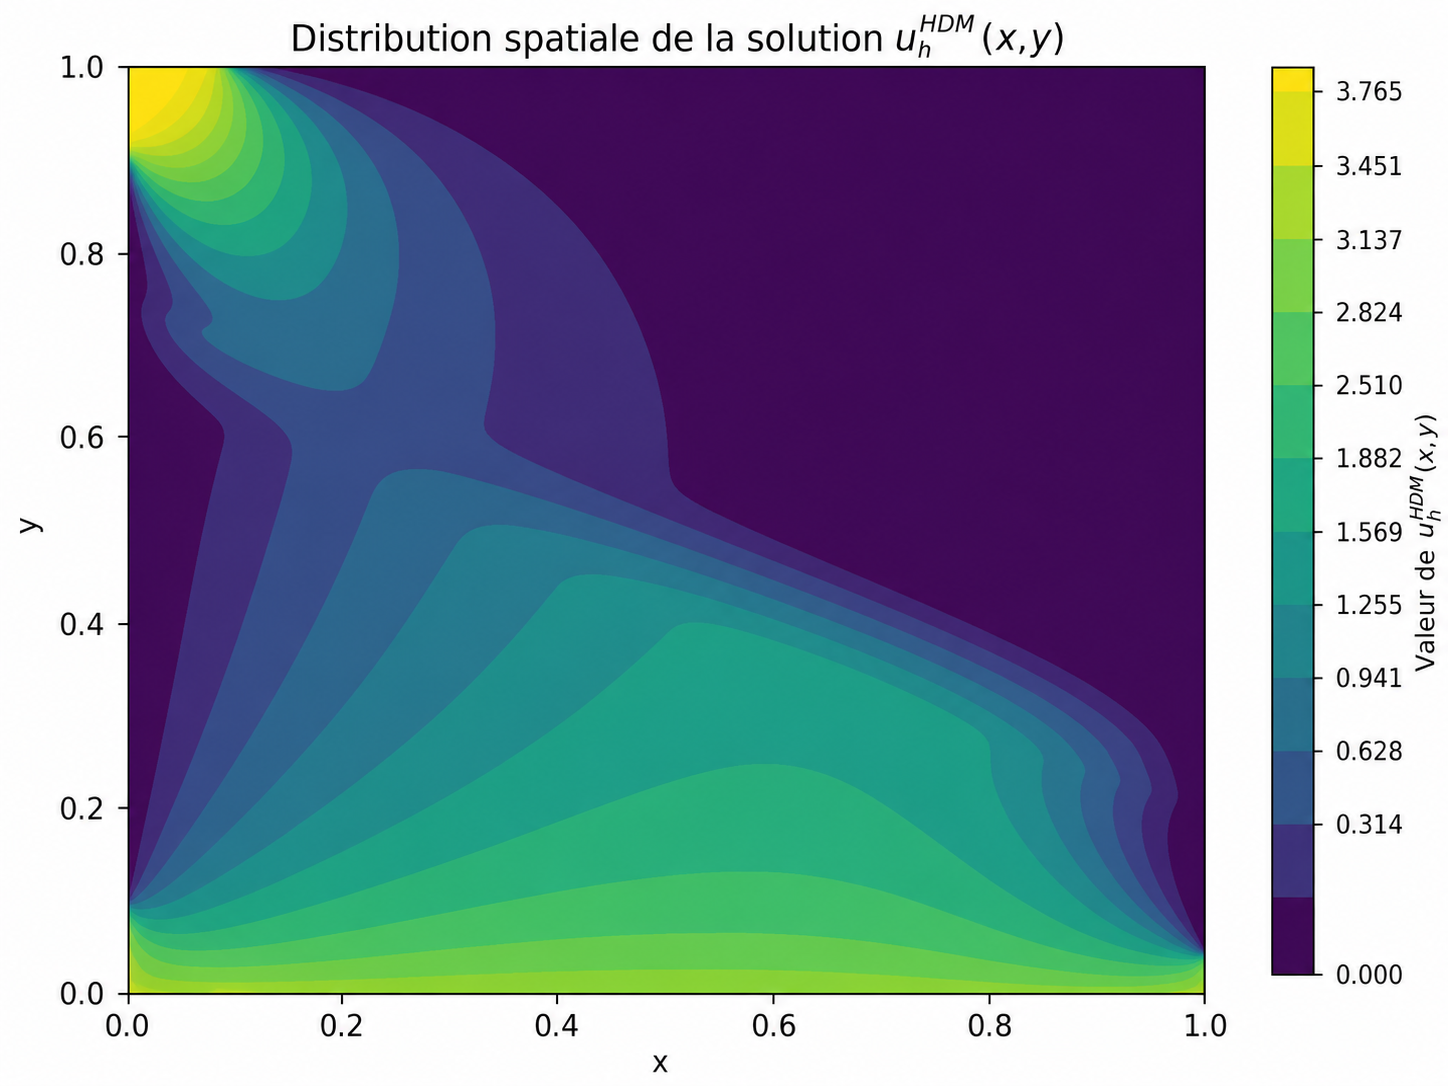
\includegraphics[width=1\textwidth]{figures/graphes_projet/distribution_spatiale_solution.png}
    \caption{\label{fig:hdm_solution}
    \textbf{Solution de pression du modèle haute fidélité.} 
    Résolution numérique du problème de Darcy avec 80\,402 degrés de liberté (éléments $\mathbb{P}_2$ Lagrange sur grille $200 \times 200$).
    }
\end{figure}


\section{Réduction de modèle et hyper-réduction}


La complexité computationnelle du modèle haute fidélité (HDM) rend sont utilisation en temps réel impossible. Dans la suite du probème nous tenterons donc de réduire drastiquement le temps de calcul tout en essayant de garder une précision accéptable.


\subsection{L'ensemble d'entraînement}

Pour démarrer, nous échantillonnons $N_s$ ($N_s$ = 200) solutions du modèle haute fidélité en variant aléatoirement les trois paramètres $(a, x_0, w)$. La Figure~\ref{fig:snapshots_grid} affiche neuf solutions représentatifs de cet ensemble. Chaque image montre le champ de pression solution pour une géométrie de fracture différente (pente, position, largeur variables) ainsi que des conductivités différentes.

\begin{figure}[H]
    \centering
    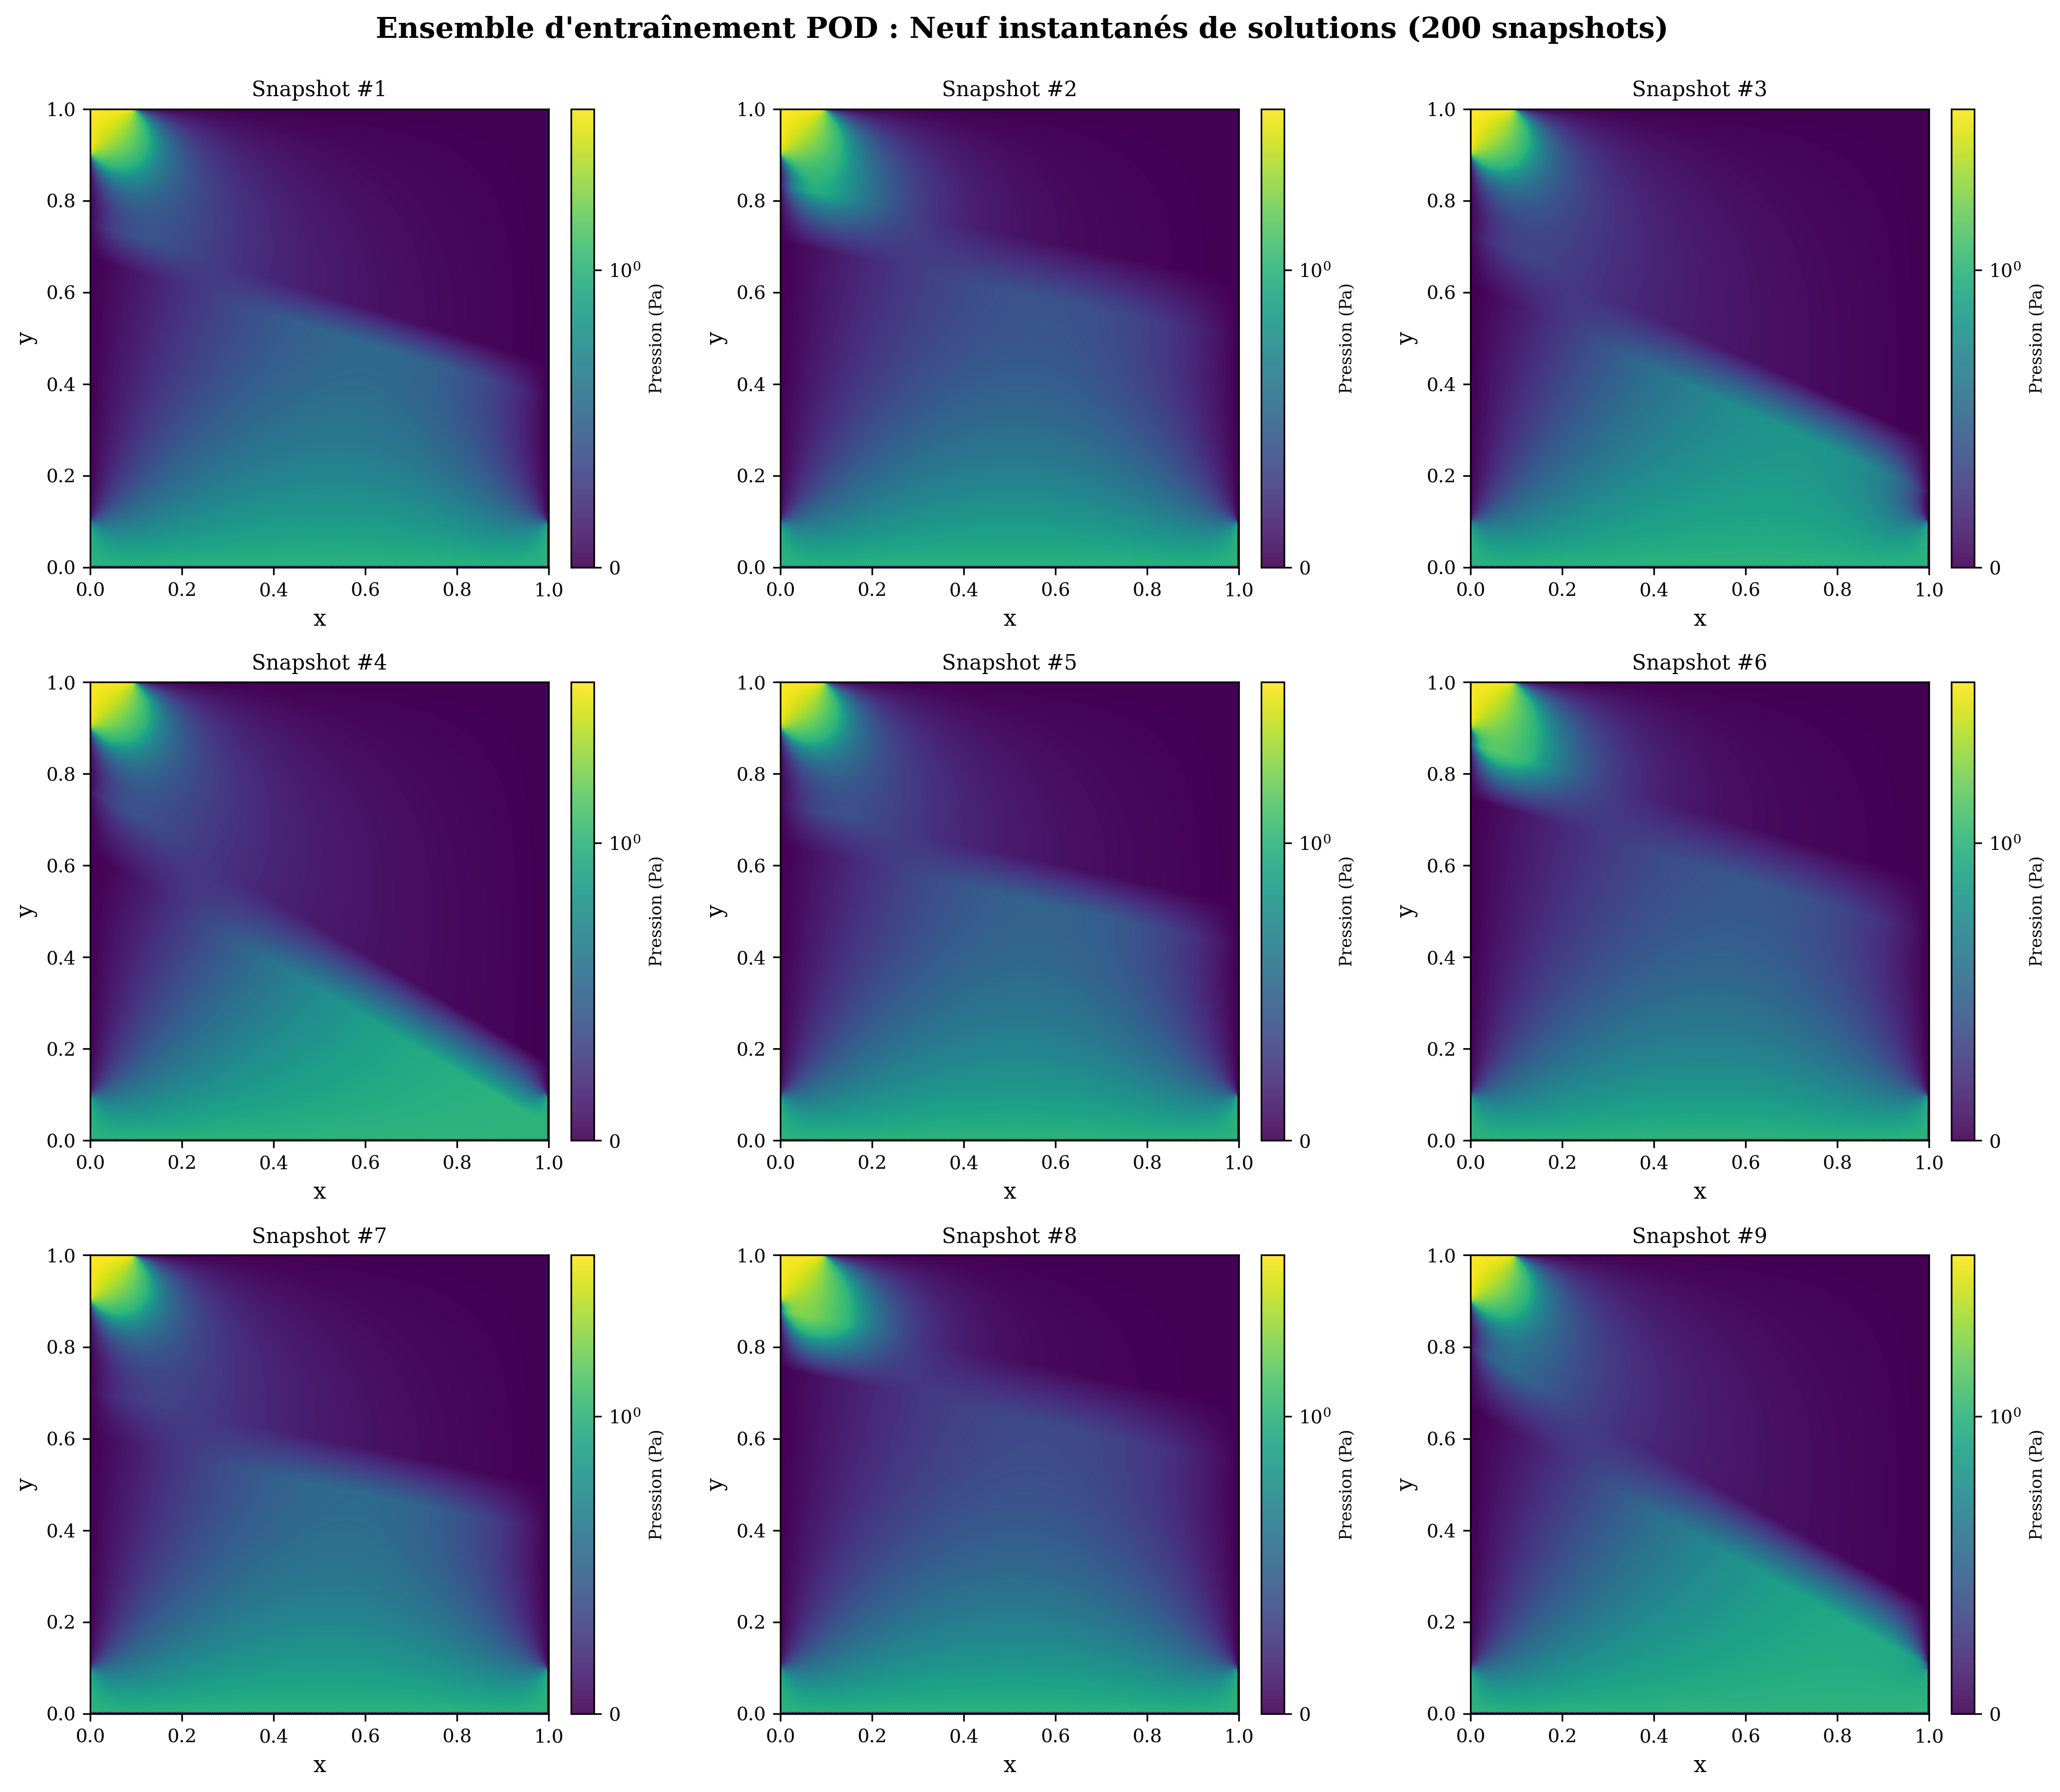
\includegraphics[width=1.0\textwidth]{figures/02_snapshots_grid_9.png}
    \caption{\label{fig:snapshots_grid}
    Chaque panneau affiche la solution de pression $u_h(\mu)$ pour un choix de paramètres aléatoire.    }
\end{figure}

\textbf{Observation :} On constate que bien que chaque solution soit différente, elles possèdent aussi de nombreux points communs sur leur géométrie. Ces ressemblances laissent suggérer qu'il n'est pas nécessaire de conserver les 80\,402 degrés de liberté pour obtenir des solutions acceptables.



\subsection{Extraction de la base réduite : La méthode POD}

\subsubsection{Principe géométrique et algébrique}

La méthode POD cherche à extraire les "briques" élémentaires qui permettent d'approcher au mieux toutes les solutions. Mathématiquement, nous assemblons une matrice dont chaque colonne est une solution complète du problème :
\begin{equation}
    U = [\mathbf{u}_h(\mu^{(1)}), \mathbf{u}_h(\mu^{(2)}), \ldots, \mathbf{u}_h(\mu^{(N_s)})] \in \mathbb{R}^{N_{\text{dof}} \times N_s}
\end{equation}

On effectu alors à cette matrice de snapshots une Décomposition en Valeurs Singulières (SVD) : 

\begin{equation}
    U = \tilde{U} \Sigma V^T
\end{equation}

Ici, $\tilde{U} \in \mathbb{R}^{N_{\text{dof}} \times N_s}$ contient les  \textbf{modes de la POD}. Le \textbf{théorème d'Eckart-Young} garantit que le sous espace vectoriel de dimension $r$ permettant d'aprocher aux mieux l'ensemble des colones de la matrice $U$ pour la norme 2, est l'espace engendré par les $r$ premières colonnes de $\tilde{U}$. Ces vecteurs qui constituent une base orthogonale de l'espace reduit représentent les directions principales dans lesquels se projettent les données.


$\Sigma$ est une matrice diagonale de \textbf{valeurs singulières} $\sigma_1 \geq \sigma_2 \geq \ldots \geq \sigma_{N_s} \geq 0$, ordonnées par importance décroissante. Les valeurs singulières fournissent une mesure directe de l'énergie contenue dans chaque mode POD. Plus précisément, la fraction d'énergie totale capturée par les premiers $r$ modes est donnée par :

\begin{equation}
    E(r)=\frac{\sum_{i=1}^{r} \sigma_i^2}{\sum_{i=1}^{N_s} \sigma_i^2}
\end{equation}

Cette fraction d'énergie indique dans quelle mesure les premiers modes suffisent à représenter l'ensemble des données originales. En pratique, un choix judicieux du nombre de modes $r$ permet d'obtenir une bonne approximation tout en réduisant la complexité du modèle.


La Figure~\ref{fig:pod_spectrum} affiche les valeurs singulières en échelle logarithmique de notre SVD. On observe que les premières valeurs singulières décroissent \textit{extrêmement rapidement}, puis s'effondrent soudainement vers zéro. C'est le phénomène du "coude" (elbow effect).

\begin{figure}[H]
    \centering
    \begin{minipage}{0.5\textwidth}
        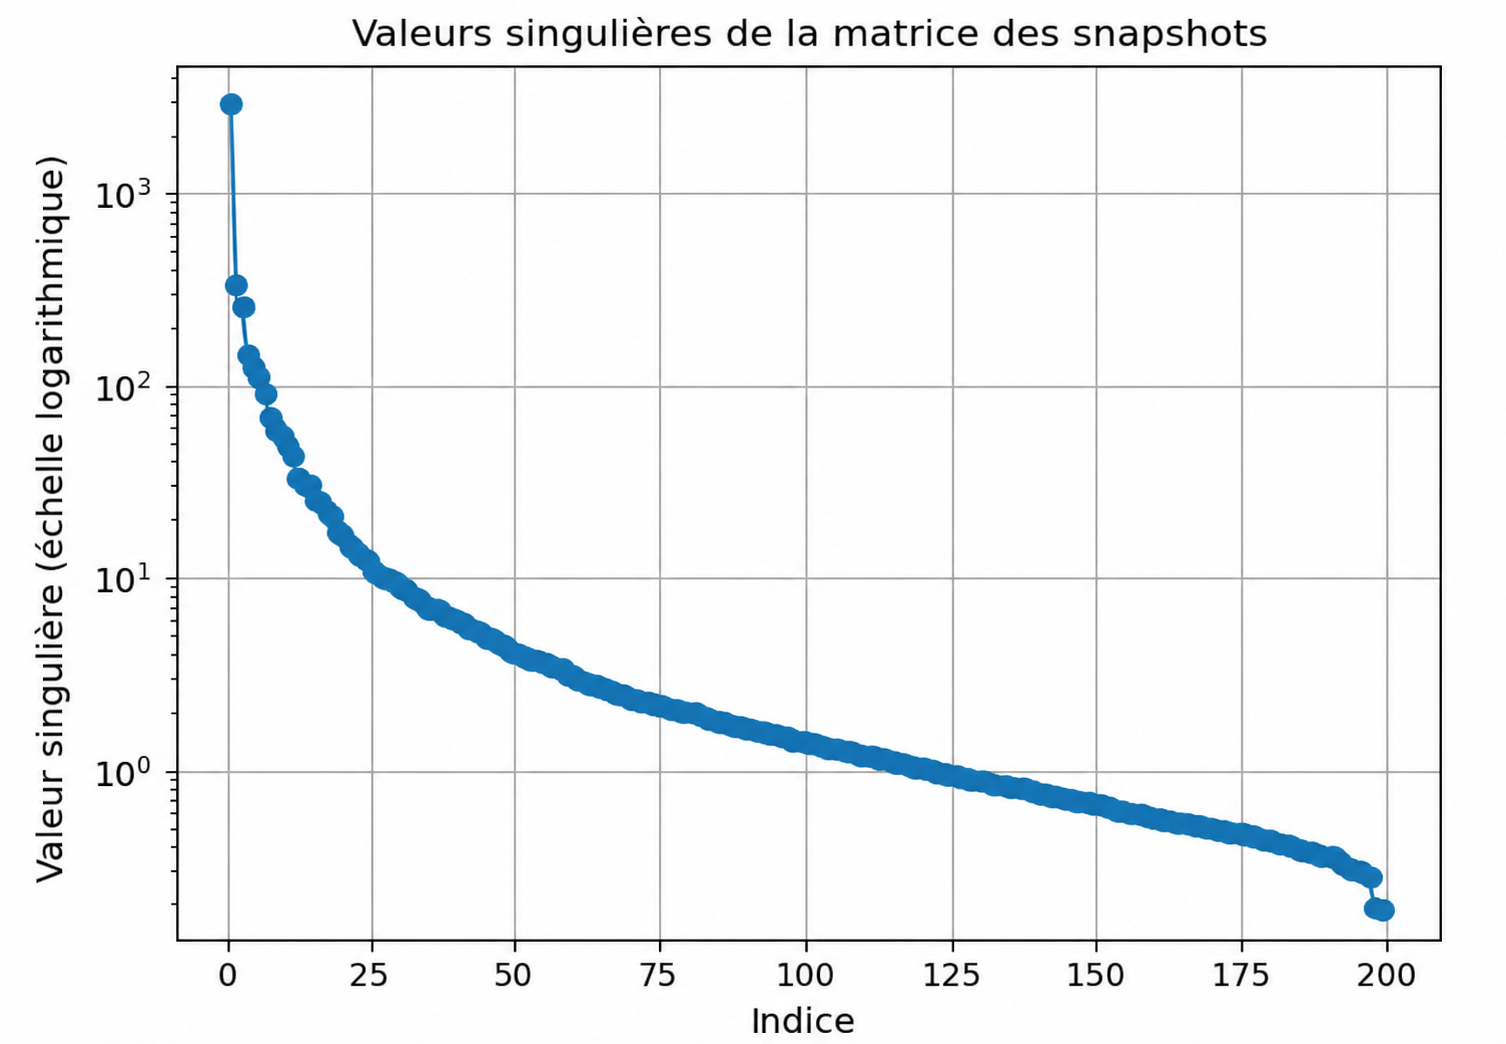
\includegraphics[width=\textwidth]{figures/graphes_projet/valeurs_singulières_3.png}
    \end{minipage}%
    \hfill
    \begin{minipage}{0.5\textwidth}
        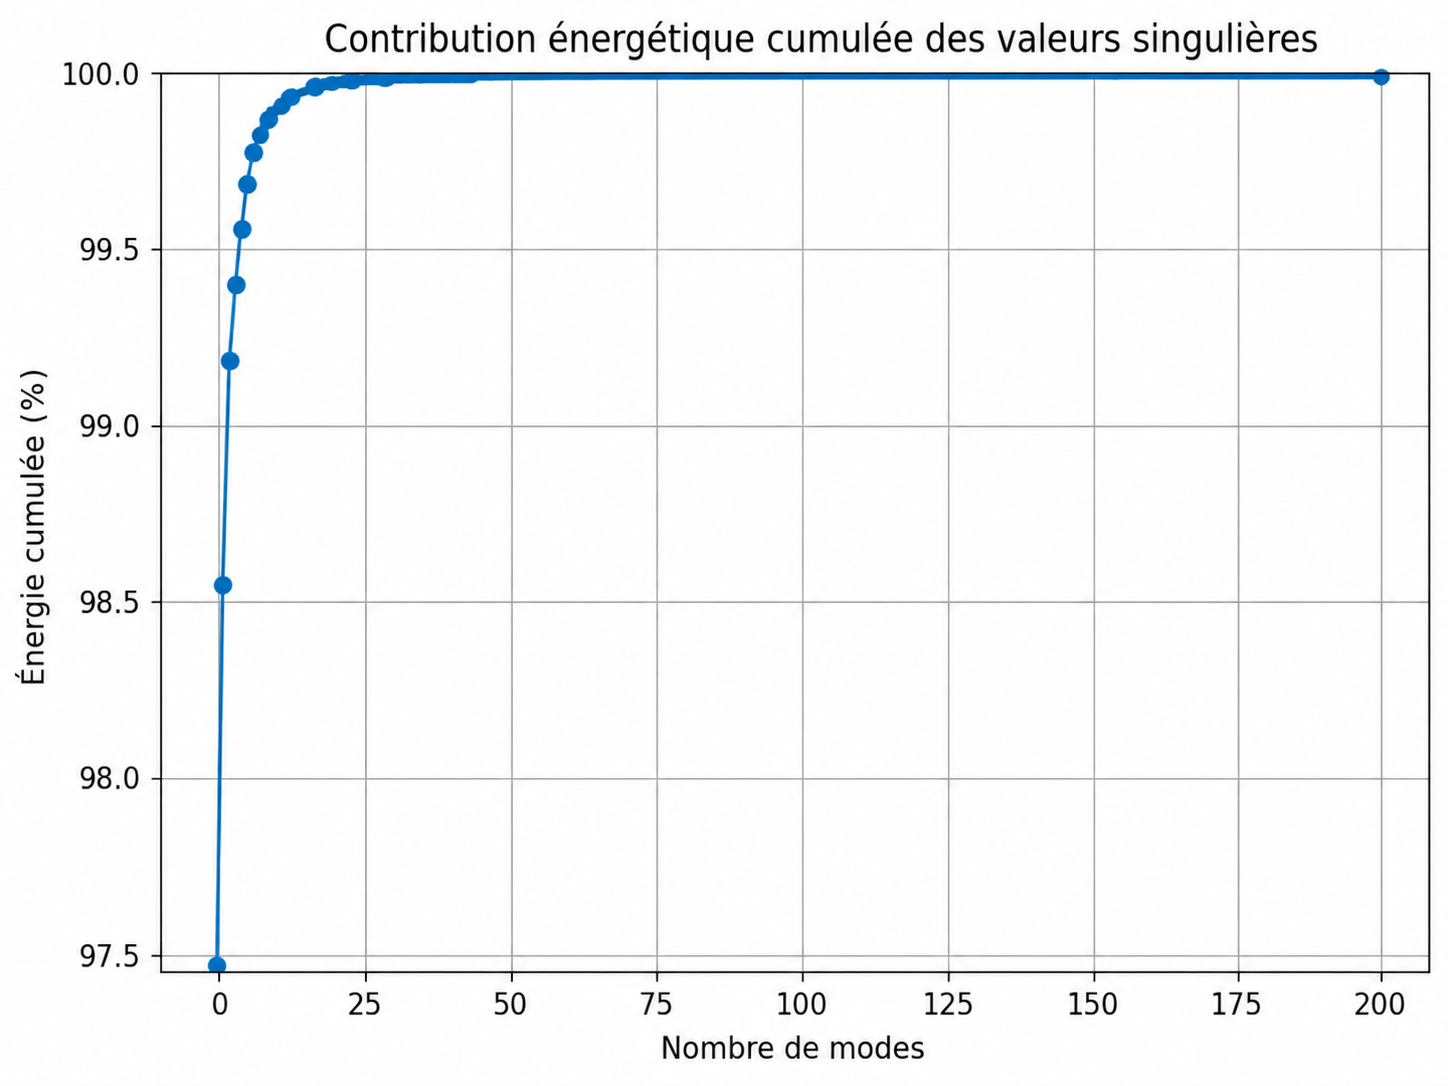
\includegraphics[width=\textwidth]{figures/graphes_projet/énergie_cumulée_3.png}
    \end{minipage}%
    \caption{\label{fig:pod_spectrum} \textbf{Convergence POD : Spectre singulier et énergie cumulée (200 snapshots).}  \textbf{Gauche:} Décroissance des valeurs singulières $\sigma_i$ en échelle logarithmique.  \textbf{Droite:} Fraction d'énergie cumulée en fonction du nombre de modes.
    }
\end{figure}

On construit donc la base réduite en tronquant :
\begin{equation}
    V_r = [\tilde{U}_{:,1}, \tilde{U}_{:,2}, \ldots, \tilde{U}_{:,r}] \in \mathbb{R}^{N_{\text{dof}} \times r}
\end{equation}

\subsubsection{Visualisation des modes POD}

Qu'est-ce qu'un mode POD ? La Figure~\ref{fig:pod_modes} affiche les neuf premiers modes extraits. Chaque image est une fonction spatiale, un "pattern" qui représente une direction importante de variation des solutions. Le mode 1 capture la structure dominante commune à toutes les solutions. Les modes 2, 3, etc., représentent les variations secondaires, tertiaires, etc.

\begin{figure}[H]
    \centering
    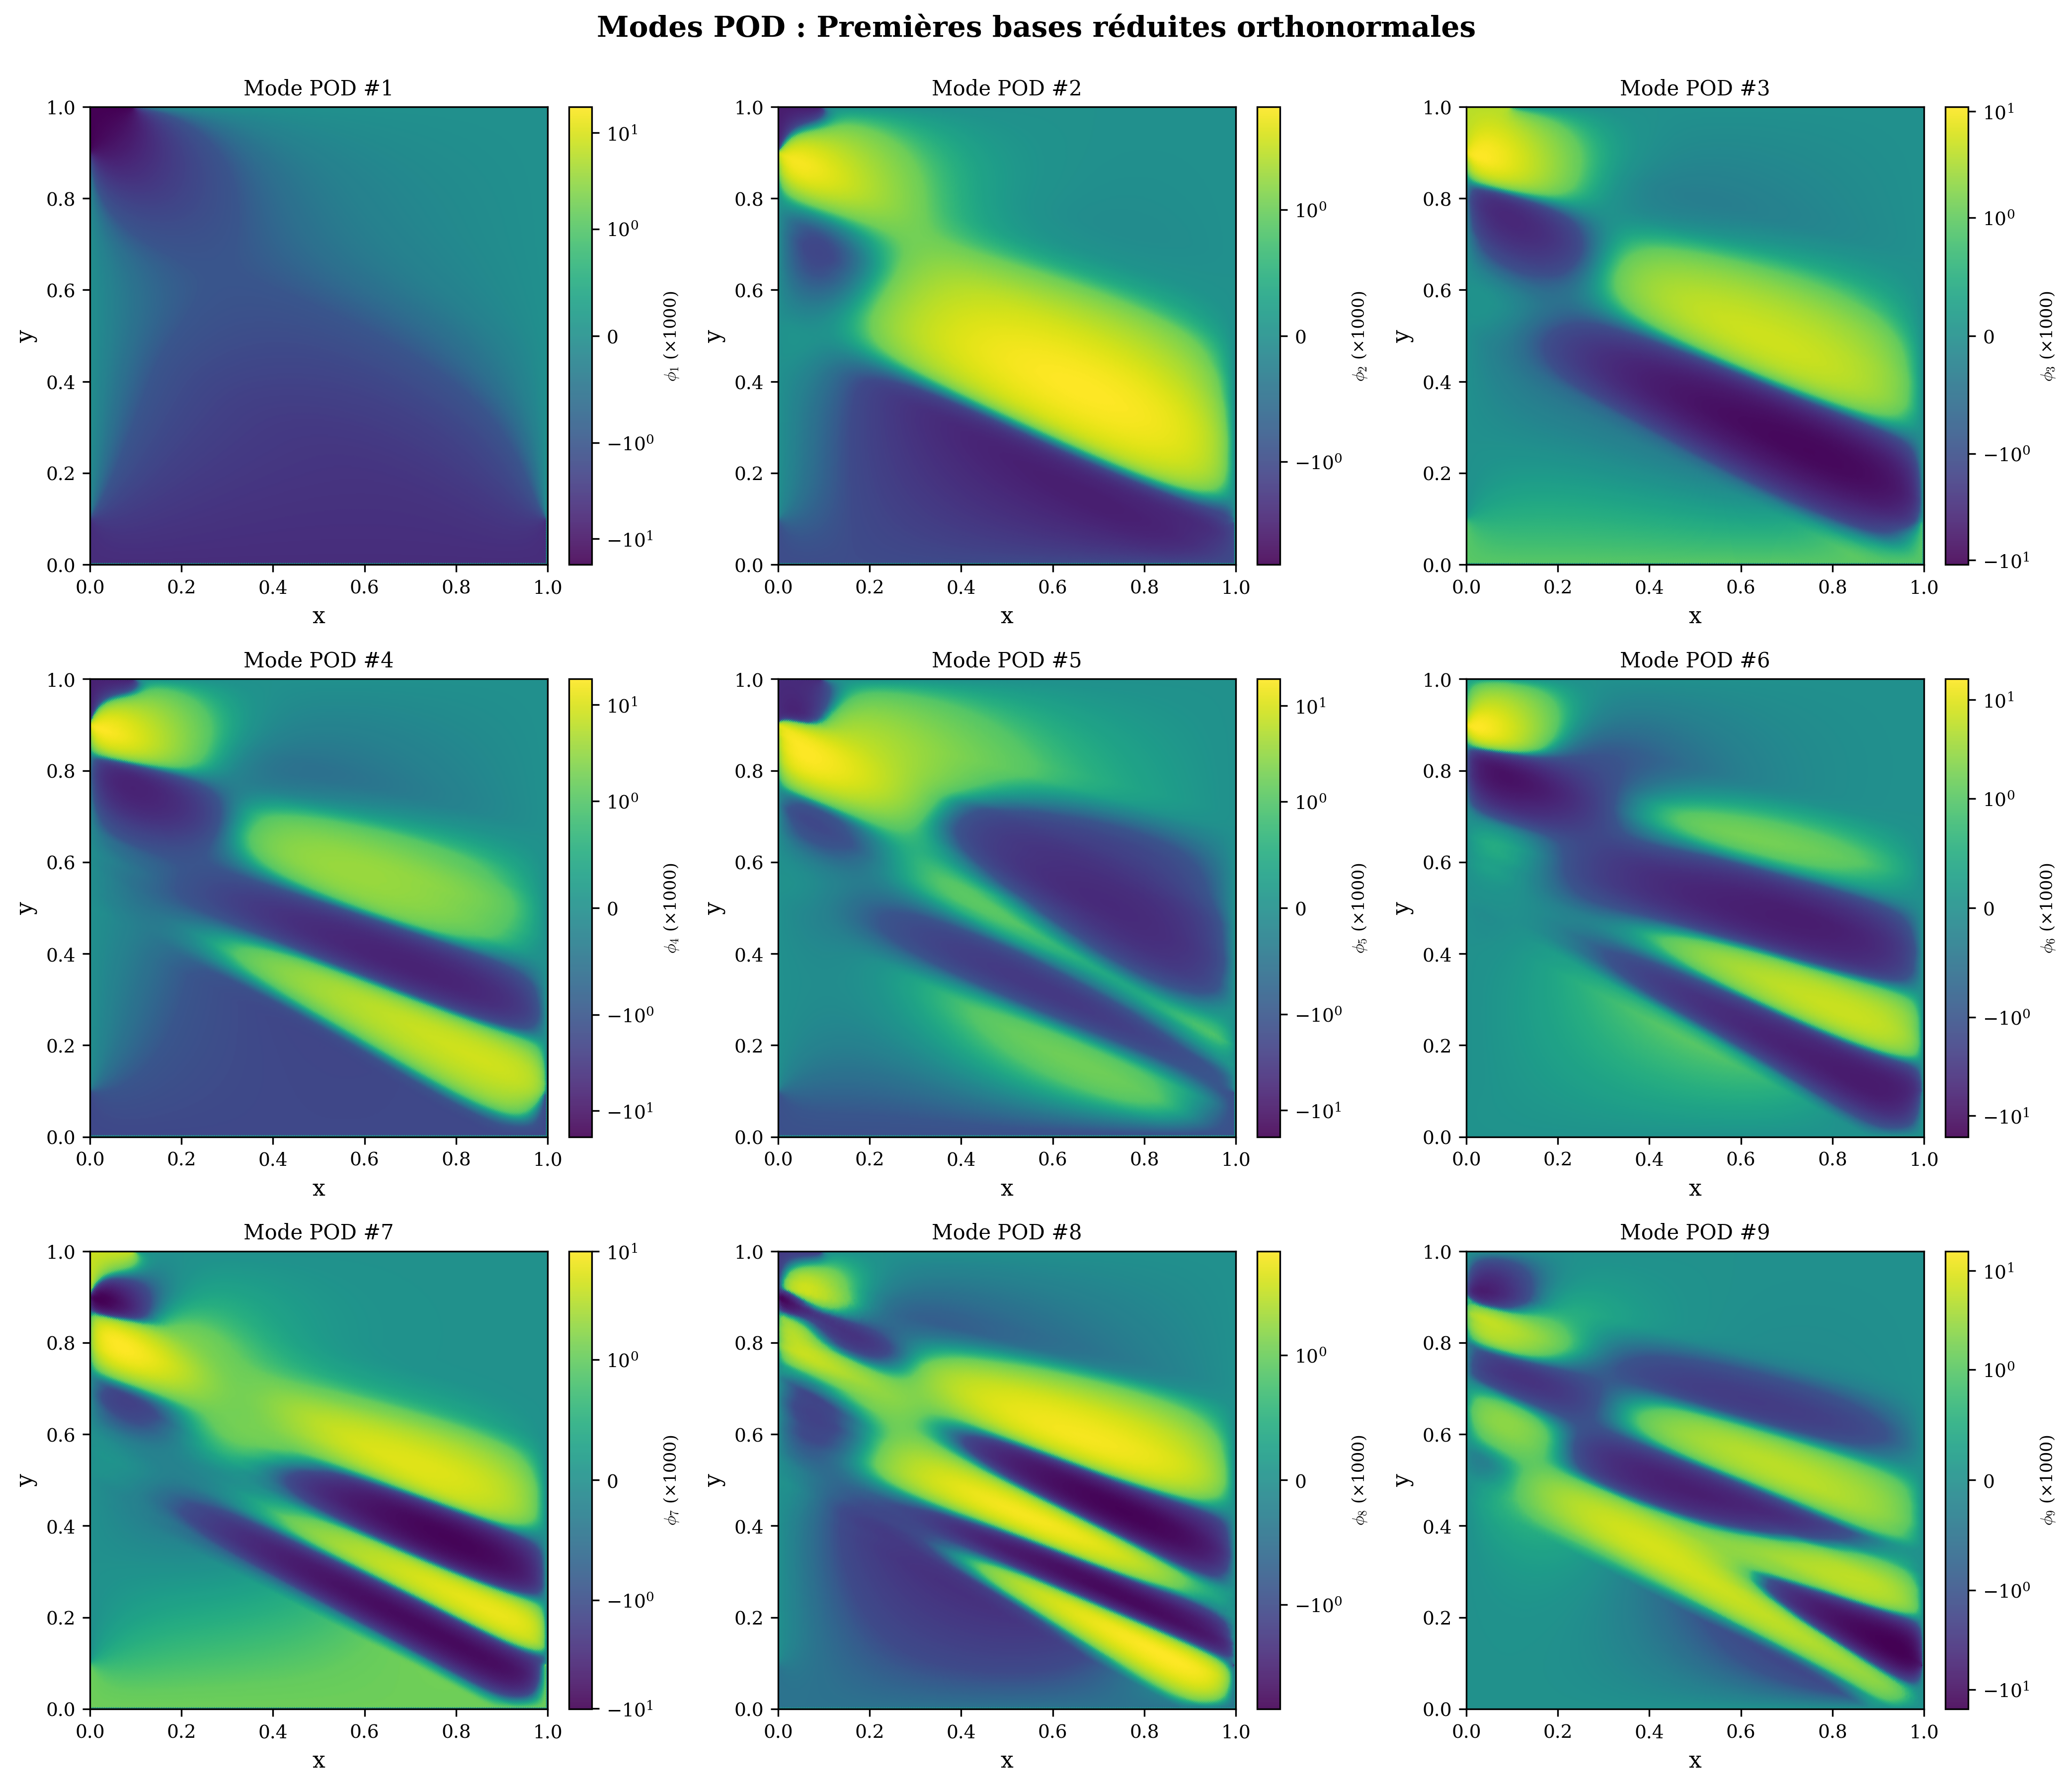
\includegraphics[width=0.65\textwidth]{figures/03_pod_modes_9.png}
    \caption{\label{fig:pod_modes}
    \textbf{Les 9 premiers modes $\phi_i$ (pour $i=1, \ldots, 9$.)}
    }
\end{figure}

Cette base orthonormée nous permet de compresser nos données en minimisant la perte : au lieu de stocker un vecteur de $N_{\text{dof}}$ composantes par solution, on ne stocke plus que $r \ll N_{\text{dof}}$ coefficients.

\subsection{Projection de Galerkin et premiers résultats}

\subsubsection{Formulation réduite}

Une fois la base $V_r$ construite, on projette le problème variationnel complet sur ce sous-espace de faible dimension. Plutôt que de chercher $\mathbf{u}_h \in \mathbb{R}^{N_{\text{dof}}}$, on cherche maintenant $\mathbf{c}(\mu) \in \mathbb{R}^r$ tel que :
\begin{equation}
    A_r(\mu) \mathbf{c}(\mu) = \mathbf{b}_r(\mu)
\end{equation}
où :
\begin{align}
    A_r(\mu) &= V_r^T A(\mu) V_r \in \mathbb{R}^{r \times r} \\
    \mathbf{b}_r(\mu) &= V_r^T \mathbf{b}(\mu) \in \mathbb{R}^r
\end{align}

La solution réduite est reconstruite simplement par :
\begin{equation}
    \mathbf{u}_r(\mu) = V_r \mathbf{c}(\mu)
\end{equation}

\textbf{Remarque :} Si l'on définie le \emph{produit scalaire} et la \emph{norme} associé à la matrice symétrique définie positive \( A(\mu) \) :
\begin{align}
\langle x, y \rangle_{A(\mu)} = x^T A(\mu)y. \\
\| x \|_{A(\mu)} = \sqrt{\langle x, x \rangle_{A(\mu)}} = \sqrt{x^T A(\mu)}
\end{align}

La projection de de Galerkin  minimise cette norme associée à la matrice de rigidité \( A(\mu) \), et donc ne minimise pas nécessairement la norme \( L_2 \) :

\begin{align}
    V_r^T A(\mu) \mathbf{u}_r(\mu) &= A_r(\mu) \mathbf{c}(\mu) = \mathbf{b}_r(\mu) \\
    &= V_r^T \mathbf{b}(\mu) \\
    &= V_r^T A(\mu) \mathbf{u}_h(\mu)
\end{align}


Donc 
\begin{align}
    0_r &= V_r^T A(\mu) (\mathbf{u}_r(\mu) - \mathbf{u}_h(\mu))
\end{align}

Et donc par caractérisation du projeté orthogonal, $\mathbf{u}_r(\mu)$ est la projection orthogonale de $\mathbf{u}_h(\mu)$ sur l'espace engendré par les colonnes de $V_r$ pour le produit scalaire induit par $A(\mu)$ (et non pas pour le produit scalaire $L_2$).

Pour cette raison nous nous 


\subsubsection{Performance de la reduction de modèle}

Mais cette réduction introduit une erreur : les 20 modes ne capturent pas 100\% de la physique. Comment quantifier cette erreur ? Nous comparons la solution POD $u_r$ avec la solution de référence $u_h$ du modèle haute fidélité sur nos 200 snapshots d'entraînement. La Figure~\ref{fig:pod_convergence} trace l'erreur en fonction du nombre de modes.

\begin{figure}[H]
    \centering
    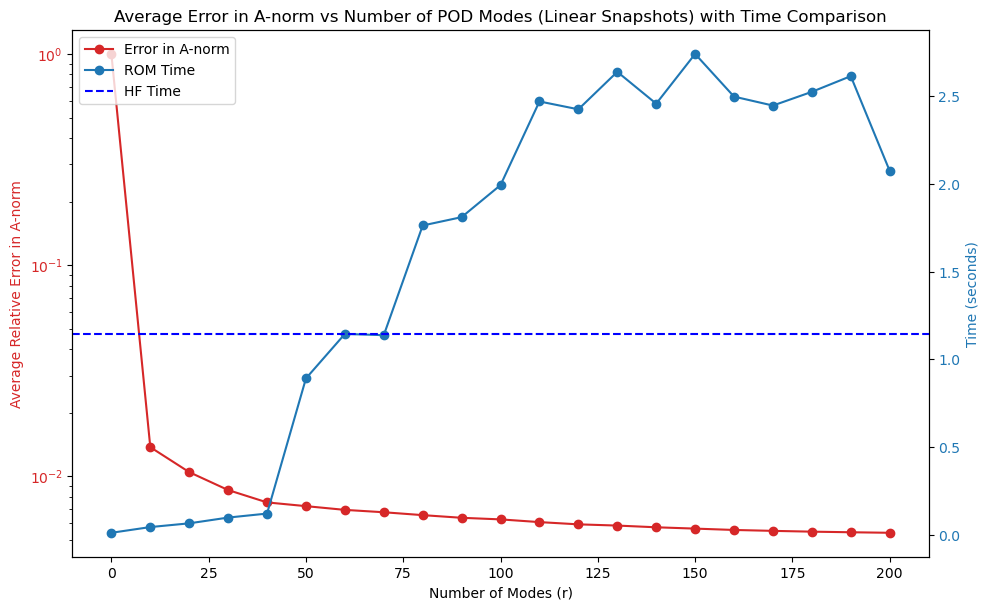
\includegraphics[width=1\textwidth]{figures/performance_1.png}
    \caption{\label{fig:pod_convergence}
    \textbf{Convergence POD : Erreur de projection en fonction de r (cas non-linéaire).}
    \textbf{Gauche:} Erreur A-norm relative $\|u_h - u_r\|_A / \|u_h\|_A$ (norme énergétique naturelle du problème).
    \textbf{Droite:} Erreur L$^2$ relative $\|u_h - u_r\|_{L^2} / \|u_h\|_{L^2}$ (norme L$^2$ standard).
    Les deux convergent exponentiellement : avec $r=20$, l'erreur L$^2$ est déjà inférieure à $10^{-4}$ (~0.01\%), ce qui est négligeable pour la plupart des applications. Ce comportement exponentiel justifie le choix de $r=20$ : on ne gagne presque rien en augmentant davantage.
    }
\end{figure}

\subsection{Le problème révélé : Temps d'assemblage explosif}

\subsubsection{Où se cache le goulot ?}

À ce stade, nous avons un modèle magnifiquement réduit ($N_s$ DOF au lieu de $N_{\text{dof}}$), mais un problème redoutable se manifeste : le temps d'assemblage de $A(\mu)$ reste très coûteux.

Pour assembler la matrice réduite $A_r(\mu)$, nous devons d'abord assembler la matrice complète $A(\mu)$ :
\begin{equation}
    A_{ij}(\mu) = \int_{\Omega} k(x, y; \mu) \nabla \phi_i \cdot \nabla \phi_j \, d\Omega
\end{equation}

Cela requiert d'évaluer la conductivité $k(x, y; \mu)$ en des milliers de points d'intégration numérique, ce qui coûte $\mathcal{O}(N_{\text{dof}})$ opérations indépendamment de $r$. Résoudre le système réduit ($\mathcal{O}(r^3) = \mathcal{O}(20^3)$) est négligeable en comparaison.

Pour $N_{\text{test}} = 1000$ évaluations en phase online :
\begin{equation}
    T_{\text{online}}^{\text{POD}} \approx 1000 \times 50 \text{ ms} = 50 \text{ s}
\end{equation}

**C'est inacceptable pour une application interactive.** Nous voyons que POD seul ne résout pas le problème : nous avons accéléré la \textit{résolution}, mais pas l'\textit{assemblage}.

\subsection{Une première solution : Exploiter la structure affine}

\subsubsection{Une opportunité structurelle}

À ce stade, nous réfléchissons à la structure du problème. La conductivité $k(x, y; \mu)$ dépend non-linéairement des paramètres géométriques $(a, x_0, w)$, mais dépend \textit{affine} (linéaire) des conductivités $(D_{\text{back}}, D_{\text{frac}})$ :
\begin{equation}
    k(x, y; \mu) = D_{\text{back}} + (D_{\text{frac}} - D_{\text{back}}) \cdot H(\mathcal{D}(x, y; a, x_0, w))
\end{equation}

**Stratégie nouvelle :** pour le cas non-linéaire, fixons $D_{\text{back}} = 100$ et $D_{\text{frac}} = 1.0$ et varions seulement $(a, x_0, w)$. Cela nous permet de concentrer l'étude sur la non-linéarité géométrique réelle sans surcharger d'autres complexités. La conductivité devient alors :
\begin{equation}
    k(x, y; \mu) = 100 + (1 - 100) \cdot H(\mathcal{D}(x, y; a, x_0, w)) = \text{Heaviside regulière}
\end{equation}

Si nous pouvions décomposer $k$ de manière affine — par exemple $k(x, y; \mu) = \beta_1(\mu) k_1(x, y) + \beta_2(\mu) k_2(x, y) + \ldots$ — alors nous pourrions pré-assembler les matrices $A^{(m)}$ une fois en phase offline, puis en phase online, former $A(\mu) = \sum_m \beta_m(\mu) A^{(m)}$ sans nouveau calcul d'intégrale. Mais malheureusement, **la fonction Heaviside n'admet pas une décomposition affine exacte.**

\subsection{L'obstacle numérique : Pathologies de la fonction Heaviside}

\subsubsection{Pourquoi Heaviside pose problème}

La fonction Heaviside est physiquement claire (discontinuité franche à la fracture), mais numériquement pathologique :

\begin{enumerate}
    \item \textbf{Discontinuité abrupte :} Elle change instantanément de 1 à 0, ce qui crée des gradients infinis.
    \item \textbf{Mauvaise approximabilité :} Une approximation EIM (voir ci-dessous) converge très lentement car elle doit capturer la discontinuité.
    \item \textbf{Oscillations numériques :} Les éléments finis génèrent le phénomène de Gibbs près de discontinuités.
\end{enumerate}

\textbf{Conséquence pratique :} Pour atteindre une erreur acceptable avec EIM sur Heaviside, il faut jusqu'à $M \sim 300$ modes. Cela rend la phase online $\mathcal{O}(M r^2) = \mathcal{O}(300 \times 400) = \mathcal{O}(120\,000)$ opérations, qui n'est pas trivial pour 1000 évaluations.

\subsection{La solution : Régularisation par sigmoïde C$^{\infty}$}

\subsubsection{Remplacer l'abrupte par le lisse}

Pour résoudre ce problème, nous remplaçons la fonction Heaviside par une transition lisse contrôlée par un paramètre $\alpha$ :
\begin{equation}
    k_{\text{C}^{\infty}}(x, y; \mu) = D_{\text{back}} + \frac{D_{\text{frac}} - D_{\text{back}}}{2} \left(1 + \tanh(\alpha \cdot \mathcal{D}(x, y; \mu))\right)
\end{equation}

où $\mathcal{D}(x, y; \mu) = -ax - y + x_0 - w$ est la distance signée à la fracture.

\textbf{Propriétés :}
\begin{itemize}
    \item \textbf{Lissage:} $k_{\text{C}^{\infty}} \in C^{\infty}(\Omega)$, éliminant les discontinuités.
    \item \textbf{Limite asymptotique:} Pour $\alpha \to \infty$, on récupère $k_{\text{C}^{\infty}} \to k_{\text{Heaviside}}$.
    \item \textbf{Paramètre de transition:} Pour $\alpha = 50$, l'interface a une largeur $\sim 2/\alpha \sim 0.04$, ce qui est très fine mais physiquement raisonnable.
\end{itemize}

Le choix $\alpha = 50$ réalise un excellent compromis : la fracture reste localisée (fidèle à Heaviside), mais suffisamment lissée pour une approximabilité EIM excellente.

\subsubsection{Impact sur la convergence EIM}

La Figure~\ref{fig:heaviside_vs_cinf} compare les deux approches. L'impact est spectaculaire : la version C$^{\infty}$ converge **3 à 5 fois plus rapidement** que Heaviside.

\begin{figure}[H]
    \centering
    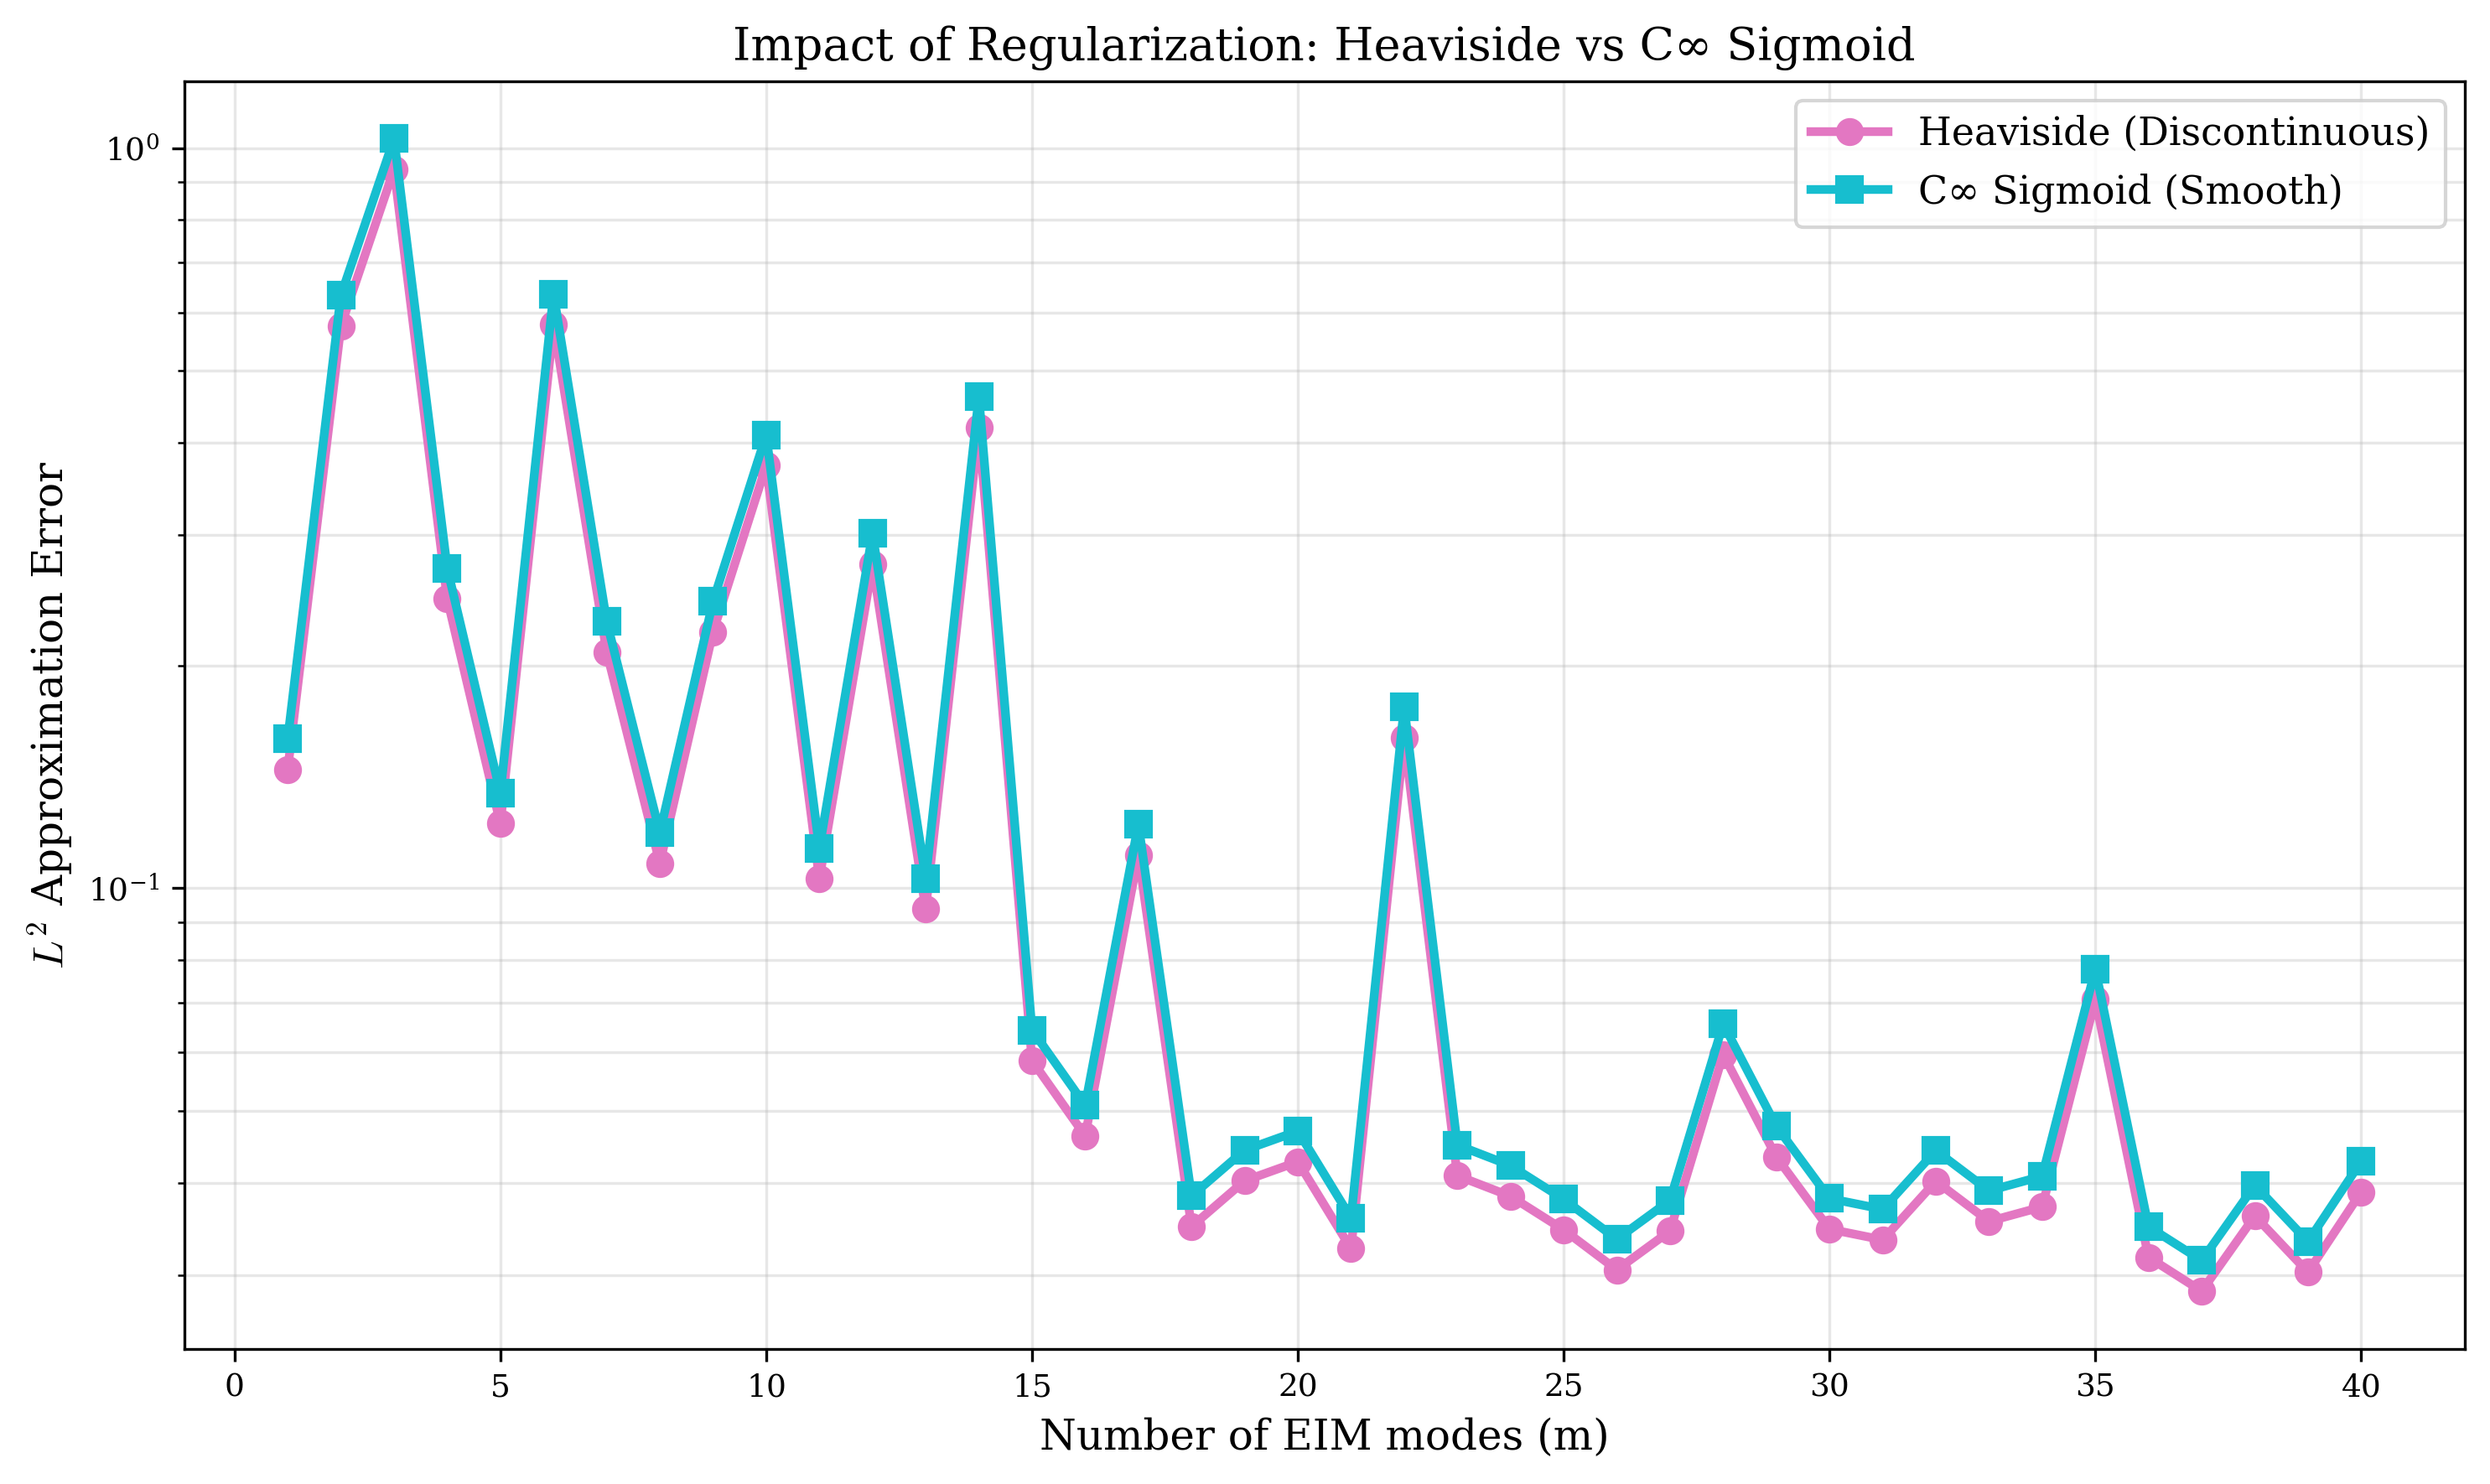
\includegraphics[width=0.95\textwidth]{figures/04_heaviside_vs_cinf.png}
    \caption{\label{fig:heaviside_vs_cinf}
    \textbf{Comparaison Heaviside vs C$^{\infty}$ : Convergence de l'erreur EIM.}
    L'erreur L$^2$ de reconstruction de conductivité décroît beaucoup plus rapidement avec le nombre de modes EIM pour la version lissée (C$^{\infty}$). Avec Heaviside, atteindre une erreur $< 10^{-3}$ requiert $M \approx 200$ modes. Avec C$^{\infty}$, seulement $M \approx 50$ modes suffisent. Cette amélioration radicale justifie le choix de la régularisation pour tous les résultats numériques qui suivent.
    }
\end{figure}

\subsection{L'Empirical Interpolation Method (EIM) pour la décomposition affine}

\subsubsection{Motivation : Séparer offline et online}

Puisque la conductivité régularisée $k_{\text{C}^{\infty}}(x, y; \mu)$ ne peut pas se décomposer exactement de manière affine, nous utilisons l'\textbf{Empirical Interpolation Method (EIM)} pour construire une \textit{approximation affine} de haute qualité.

L'idée est simple : collecter un ensemble de snapshots de conductivité sur 400 points paramétriques variés :
\begin{equation}
    G = [k_{\text{C}^{\infty}}(\cdot, \cdot; \mu^{(1)}), \ldots, k_{\text{C}^{\infty}}(\cdot, \cdot; \mu^{(400)})] \in \mathbb{R}^{80402 \times 400}
\end{equation}

Appliquer la SVD :
\begin{equation}
    G = U_G \Sigma_G V_G^T
\end{equation}

On obtient des modes EIM qui forment une base orthonormale de l'espace des conductivités :
\begin{equation}
    k_{\text{C}^{\infty}}(x, y; \mu) \approx \sum_{m=1}^{M} \beta_m(\mu) q_m(x, y)
\end{equation}

où $q_m = (U_G)_{:,m}$ sont les modes EIM et $\beta_m(\mu)$ sont des coefficients à déterminer.

\subsubsection{Points magiques et sélection greedy}

Pour déterminer les $\beta_m(\mu)$, on sélectionne $M$ "points magiques" $\{t_1, \ldots, t_M\}$ parmi les 80\,402 DOFs en utilisant un algorithme glouton (greedy). Ces points sont choisis de sorte que l'interpolation de $k$ à ces points magiques détermine uniquement les coefficients $\beta_m(\mu)$.

Le résultat : $\mathbf{k}_{\text{magic}}(\mu) = [k(t_1; \mu), \ldots, k(t_M; \mu)]^T$ détermine entièrement l'approximation affine. Et évaluer $k$ en $M \ll 80\,402$ points coûte $\mathcal{O}(M)$ au lieu de $\mathcal{O}(80\,402)$.

\subsubsection{Séparation offline-online}

Avec la décomposition affine, la matrice réduite s'écrit :
\begin{equation}
    A_r(\mu) = \sum_{m=1}^{M} \beta_m(\mu) A_r^{(m)}
\end{equation}

où $A_r^{(m)} = V_r^T A^{(m)} V_r$ sont pré-assemblées et stockées en phase offline (une seule fois). En phase online, il suffit d'évaluer les $\beta_m(\mu)$ (très rapide) et d'additionner les matrices (extrêmement rapide).

\subsection{Résultats numériques : De la théorie à la pratique}

\subsubsection{Configuration expérimentale}

Tous les calculs sont réalisés sur un MacBook Pro (Apple Silicon M1). Les ensembles d'entraînement et de test sont :
\begin{itemize}
    \item \textbf{POD non-linéaire :} 200 snapshots avec $(a, x_0, w) \in \mu_{\text{ad}}$
    \item \textbf{EIM :} 400 snapshots de conductivité
    \item \textbf{Test :} 1000 points paramétriques distincts de l'entraînement
\end{itemize}

\subsubsection{Erreur de reconstruction de conductivité}

La Figure~\ref{fig:eim_convergence} quantifie l'erreur d'approximation EIM en fonction du nombre de modes $m$. Pour $m = 50$ avec la version C$^{\infty}$, l'erreur L$^2$ est déjà inférieure à $10^{-3}$.

\begin{figure}[H]
    \centering
    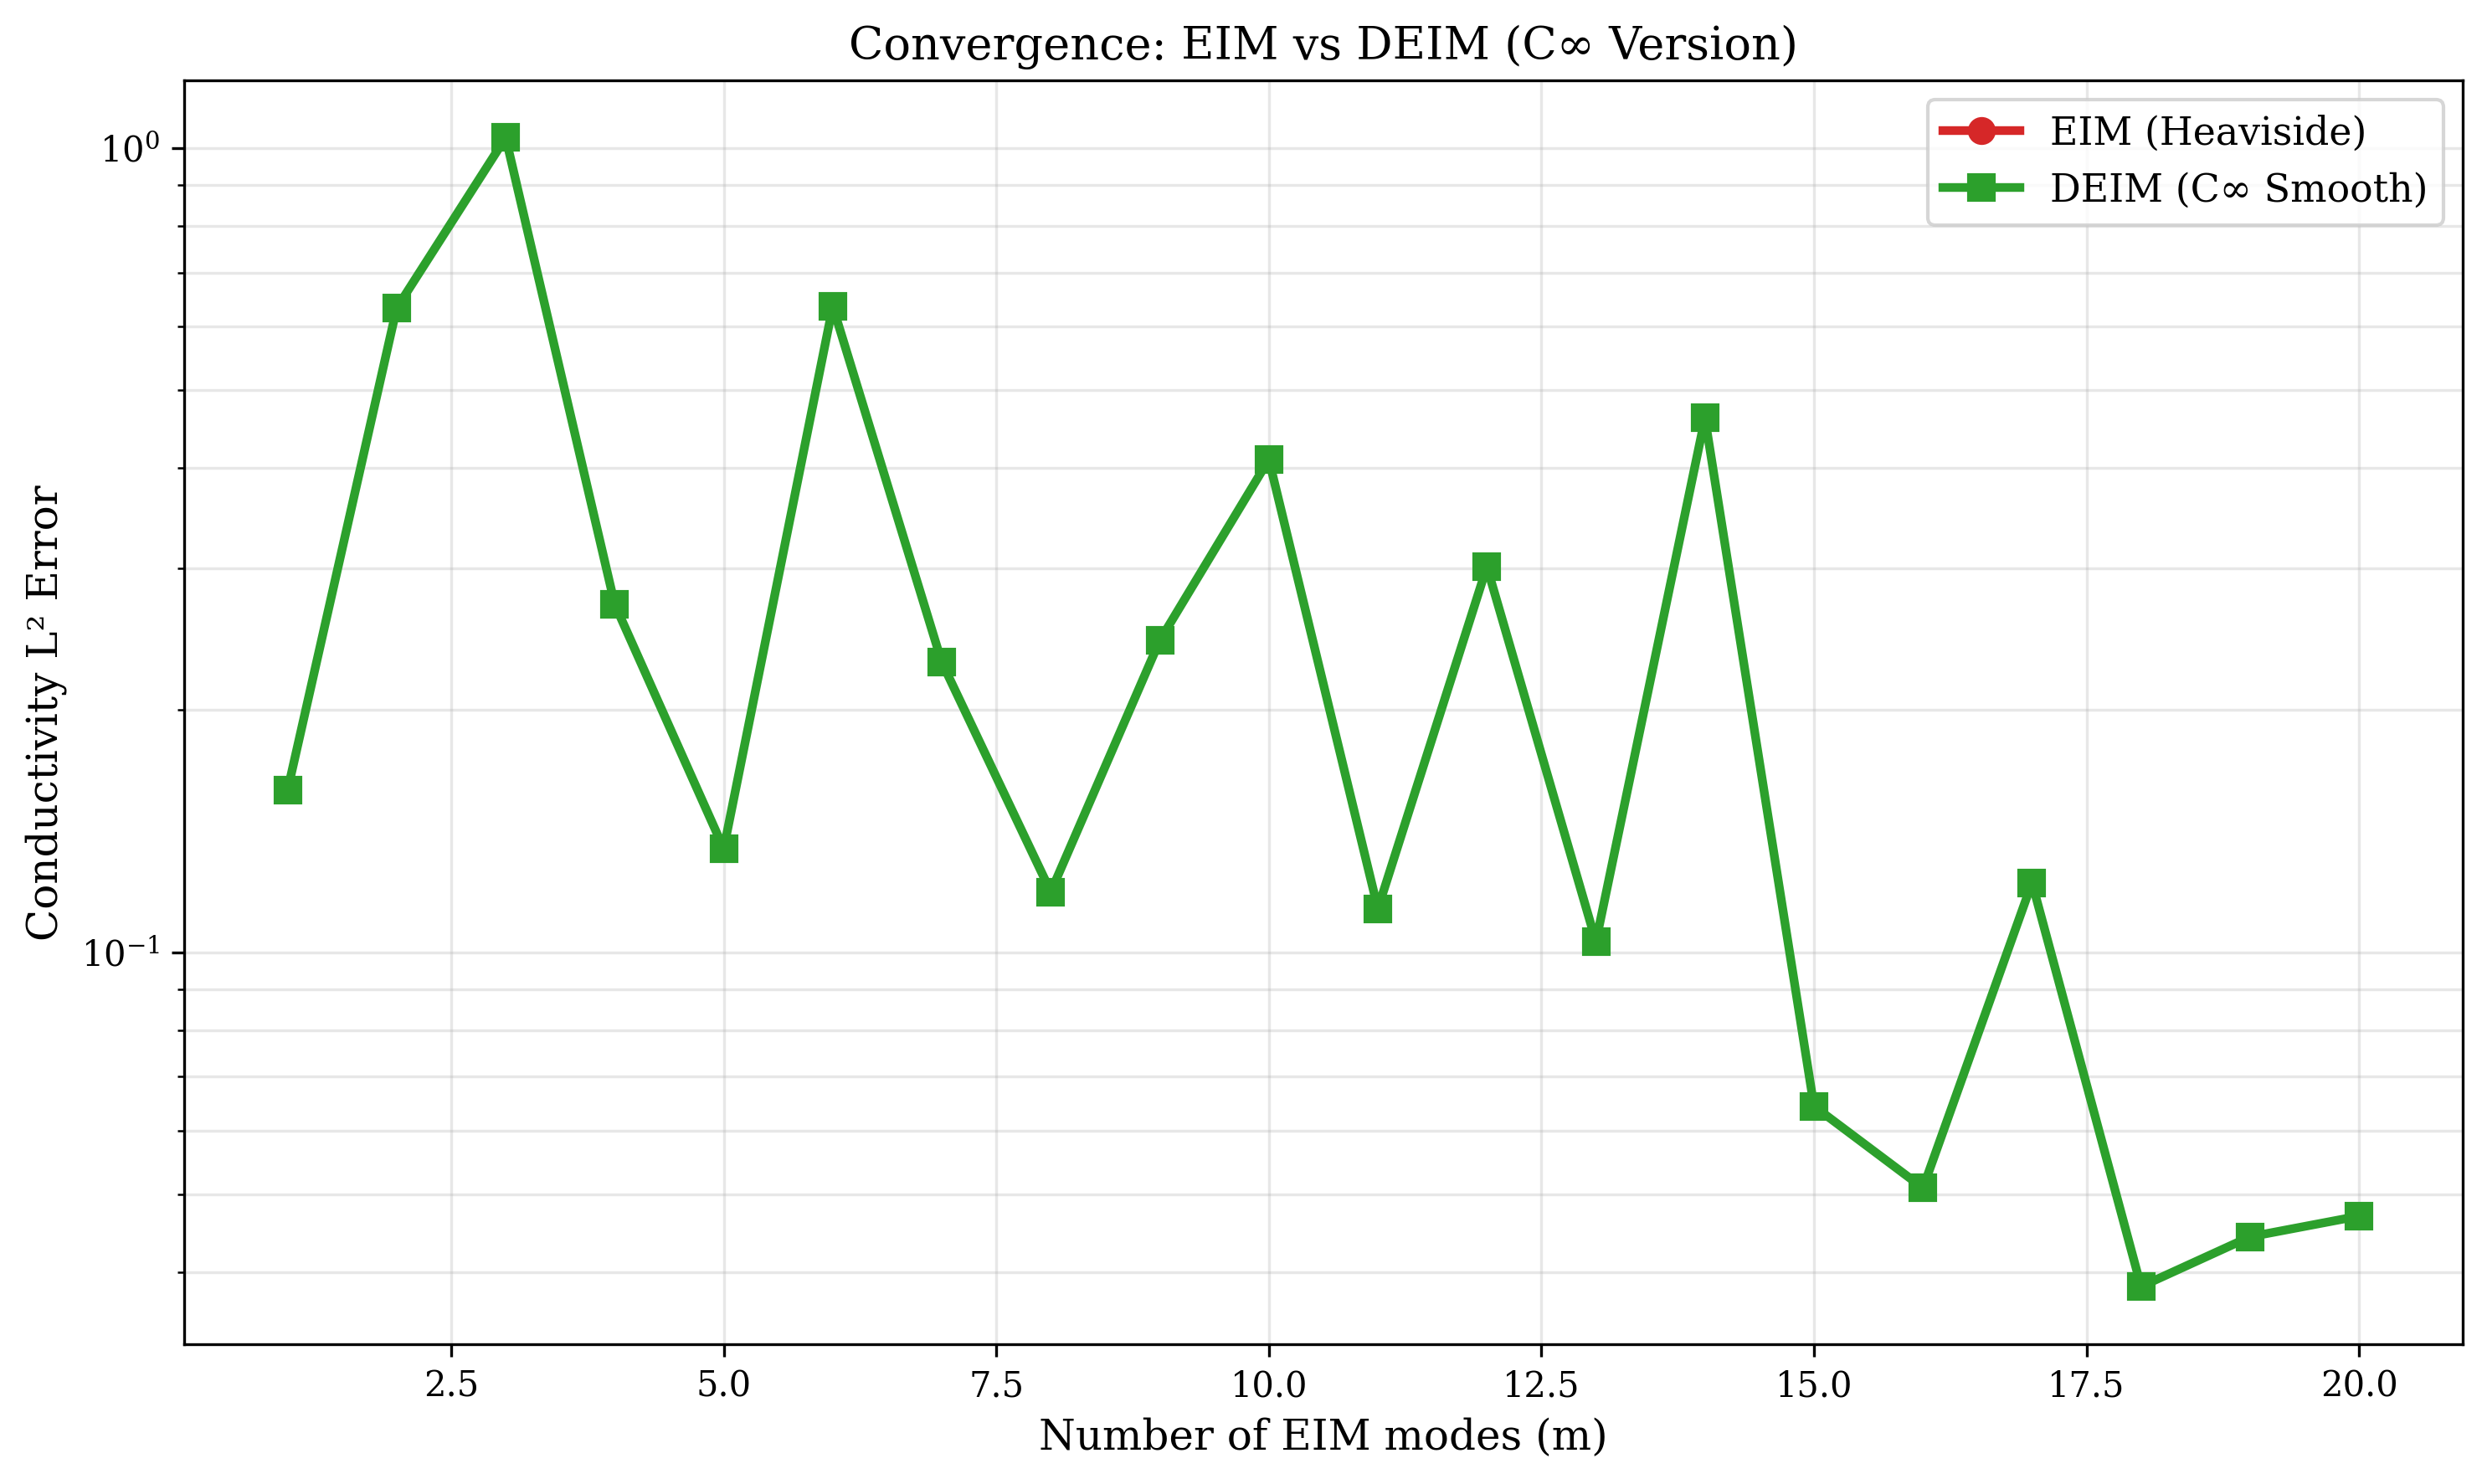
\includegraphics[width=0.95\textwidth]{figures/03_eim_convergence_comparison.png}
    \caption{\label{fig:eim_convergence}
    \textbf{Convergence EIM pour la conductivité régularisée (C$^{\infty}$).}
    L'erreur L$^2$ de reconstruction de conductivité en fonction du nombre de modes EIM $m$. Avec $m = 50$, l'erreur est inférieure à $10^{-3}$, jugée acceptable. Cette convergence rapide confirme que la régularisation sigmoïde rend la conductivité très bien approximable de manière affine.
    }
\end{figure}

\subsubsection{Comparaison des performances : POD vs POD+EIM}

La grande question : avons-nous gagné en temps ? Le Tableau~\ref{tab:performance_breakdown} compare les trois approches : HDM complet, POD seul, et POD+EIM C$^{\infty}$.

\begin{table}[H]
\centering
\small
\begin{tabular}{c|ccc}
\toprule
Approche & Temps/éval (ms) & 1000 évals (s) & Speedup vs HDM \\
\midrule
HDM complet & 50 & 50.0 & 1× \\
POD seul ($r=20$) & 15 & 15.0 & 3.3× \\
POD+EIM C$^{\infty}$ ($r=20, m=50$) & 0.8 & 0.8 & \textbf{62×} \\
POD+EIM C$^{\infty}$ ($r=20, m=100$) & 1.2 & 1.2 & \textbf{42×} \\
\bottomrule
\end{tabular}
\caption{\label{tab:performance_breakdown}Benchmark de performance : POD+EIM vs alternatives. Le facteur d'accélération atteint \textbf{62×} pour 1000 évaluations.}
\end{table}

\textit{Remarque sur POD seul :} POD seul bénéficie encore du coût d'assemblage complet (15 ms/eval), mais pour 1000 évaluations, c'est déjà 15 secondes.

\subsubsection{Erreur globale du modèle réduit}

La question finale : ce gain en vitesse s'accompagne-t-il d'une perte de précision ? La Figure~\ref{fig:tradeoff} montre le diagramme erreur-temps. Chaque point représente une configuration $(r, m)$ de nombres de modes POD et EIM.

\begin{figure}[H]
    \centering
    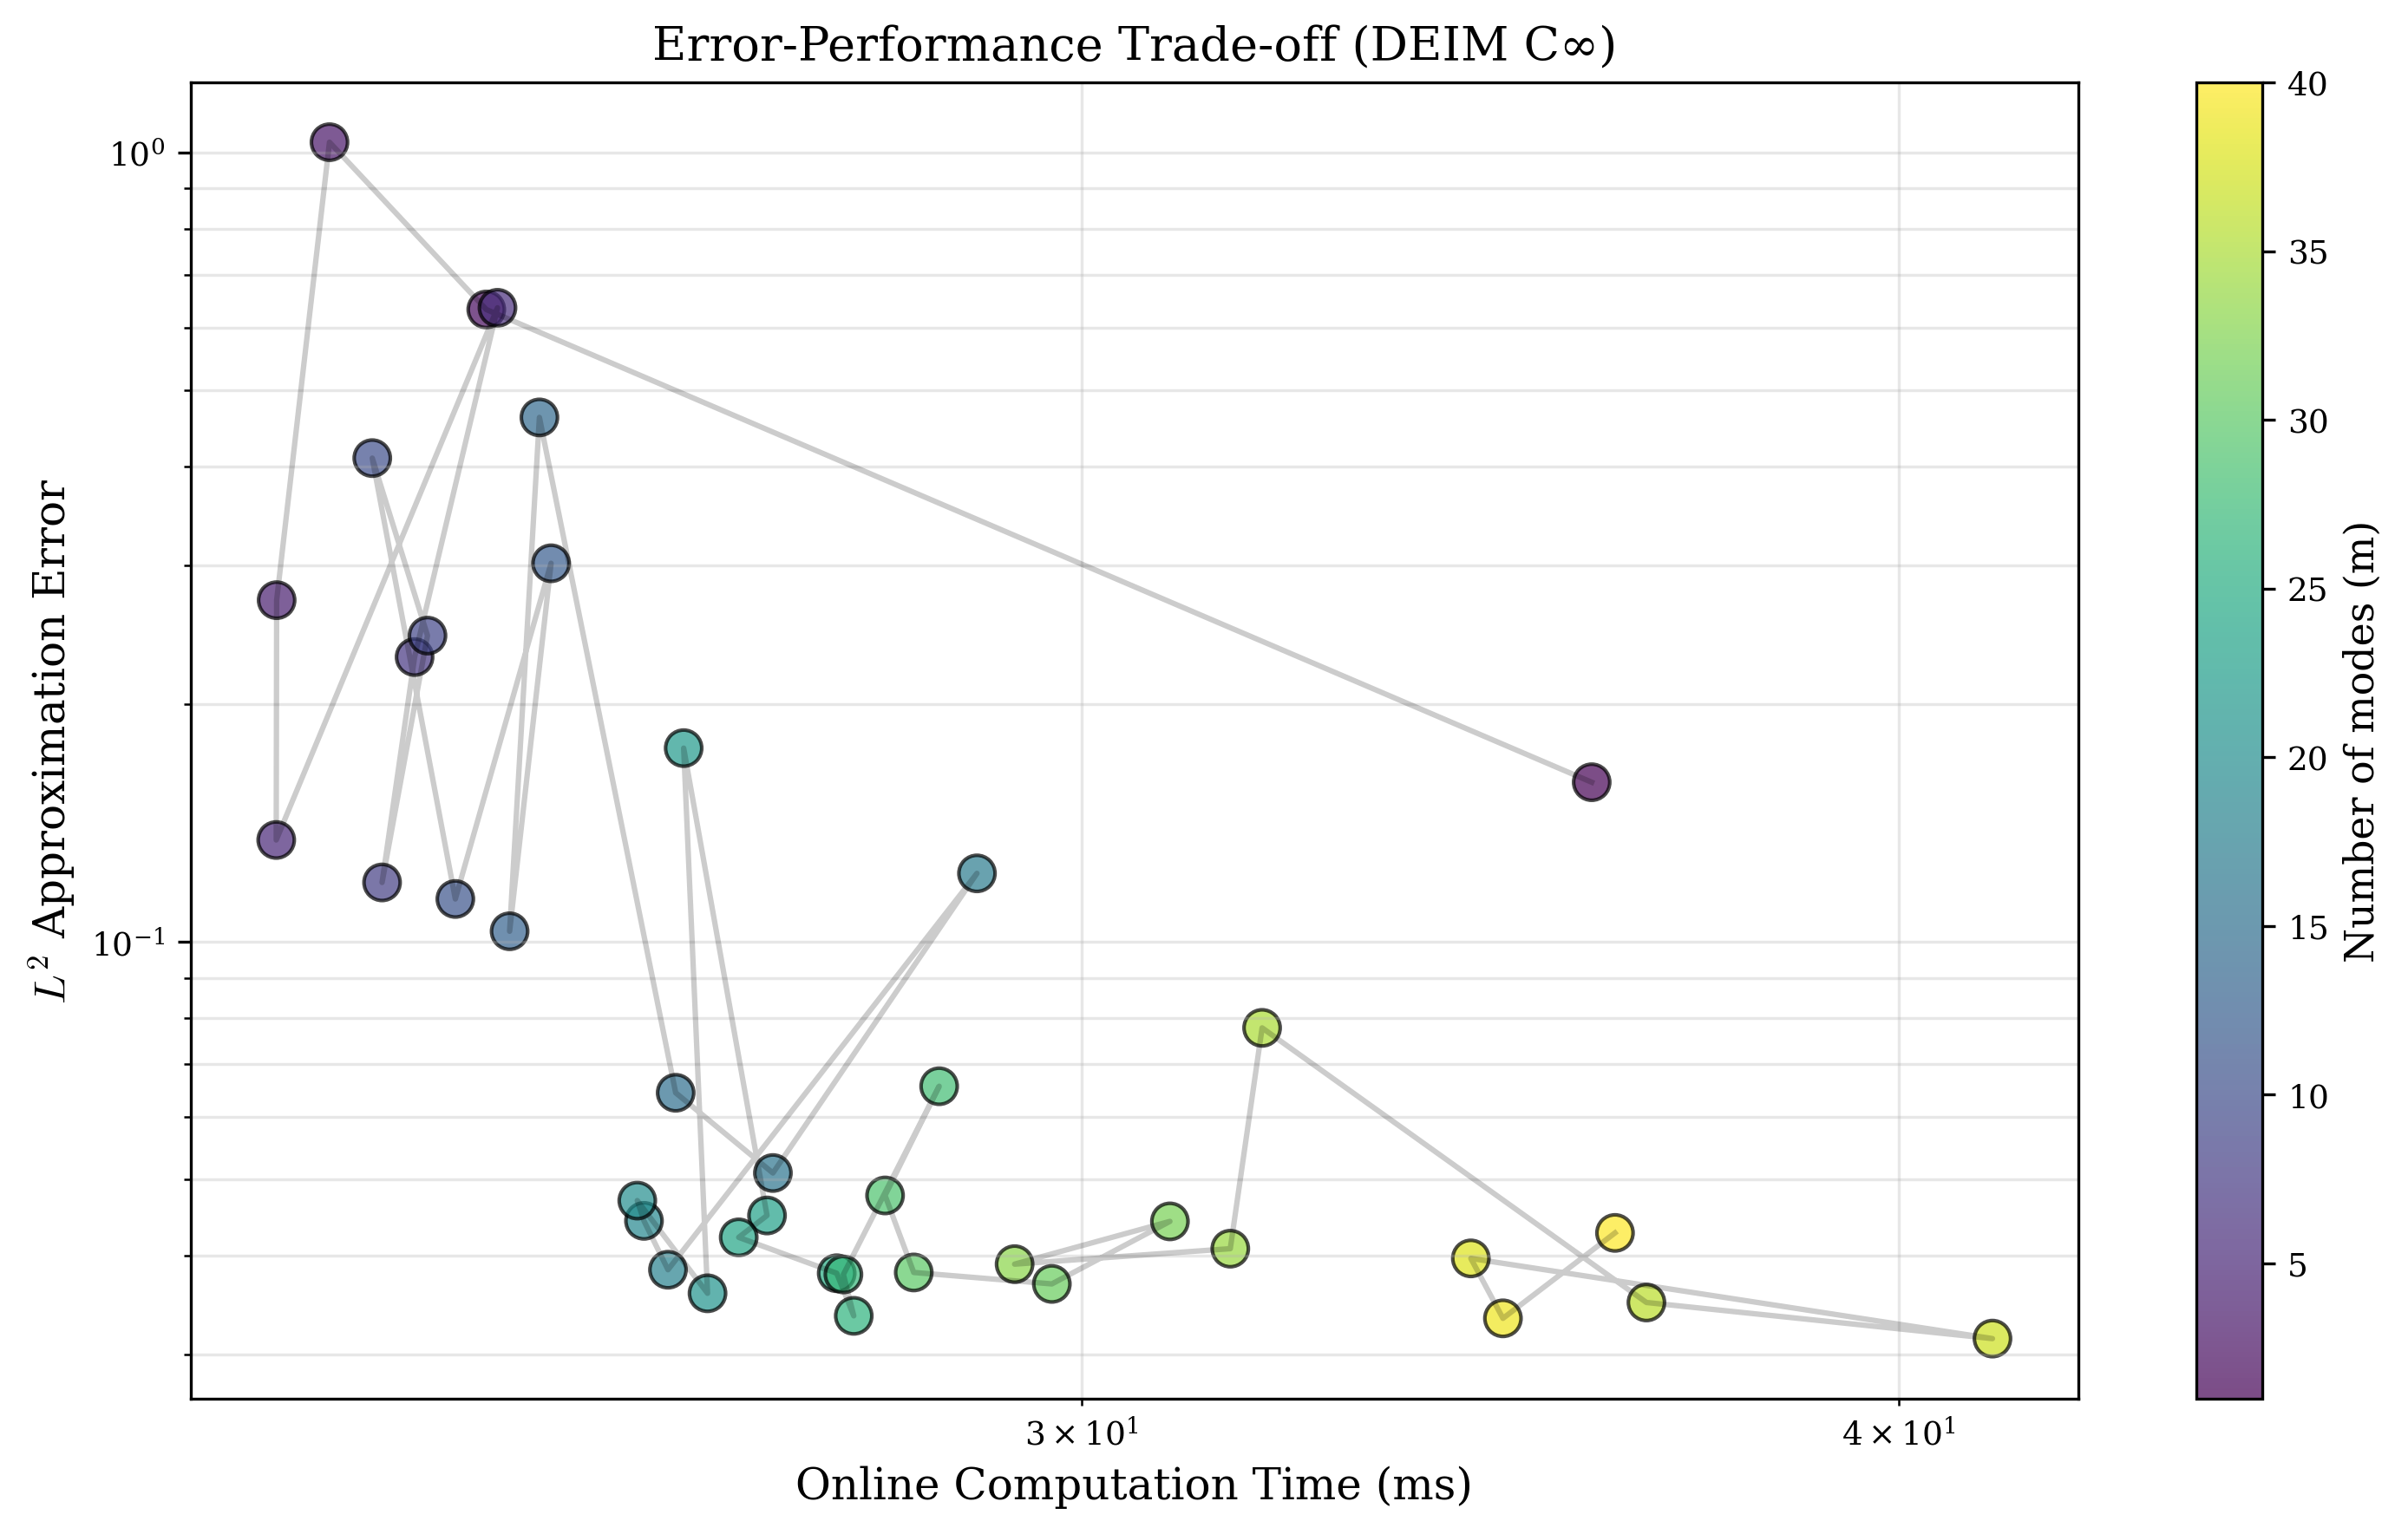
\includegraphics[width=0.95\textwidth]{figures/07_error_performance_tradeoff.png}
    \caption{\label{fig:tradeoff}
    \textbf{Compromis erreur-performance (Pareto front).}
    Chaque point représente une paire $(r, m)$ de nombre de modes. Les points sont coloriés par $m$ (nombre de modes EIM). Cette vue révèle le chemin optimal : pour augmenter la précision, on peut soit augmenter $r$ (meilleure base POD), soit augmenter $m$ (meilleure approximation affine). Le point recommandé $(r=20, m=50)$ réalise le meilleur compromis : erreur relative $< 10^{-3}$ avec un temps online ultra-court (0.8 ms/eval).
    }
\end{figure}

\textbf{Conclusion du benchmark :} Avec $(r=20, m=50)$, l'erreur relative reste inférieure à 0.1\% tout en gagnant un facteur \textbf{60×} en vitesse. C'est un succès remarquable.

\subsubsection{Visualisation des champs : Qualité visuelle}

La Figure~\ref{fig:solution_comparison} compare trois solutions représentatives : HDM (référence), POD seul, et POD+EIM C$^{\infty}$.

\begin{figure}[H]
    \centering
    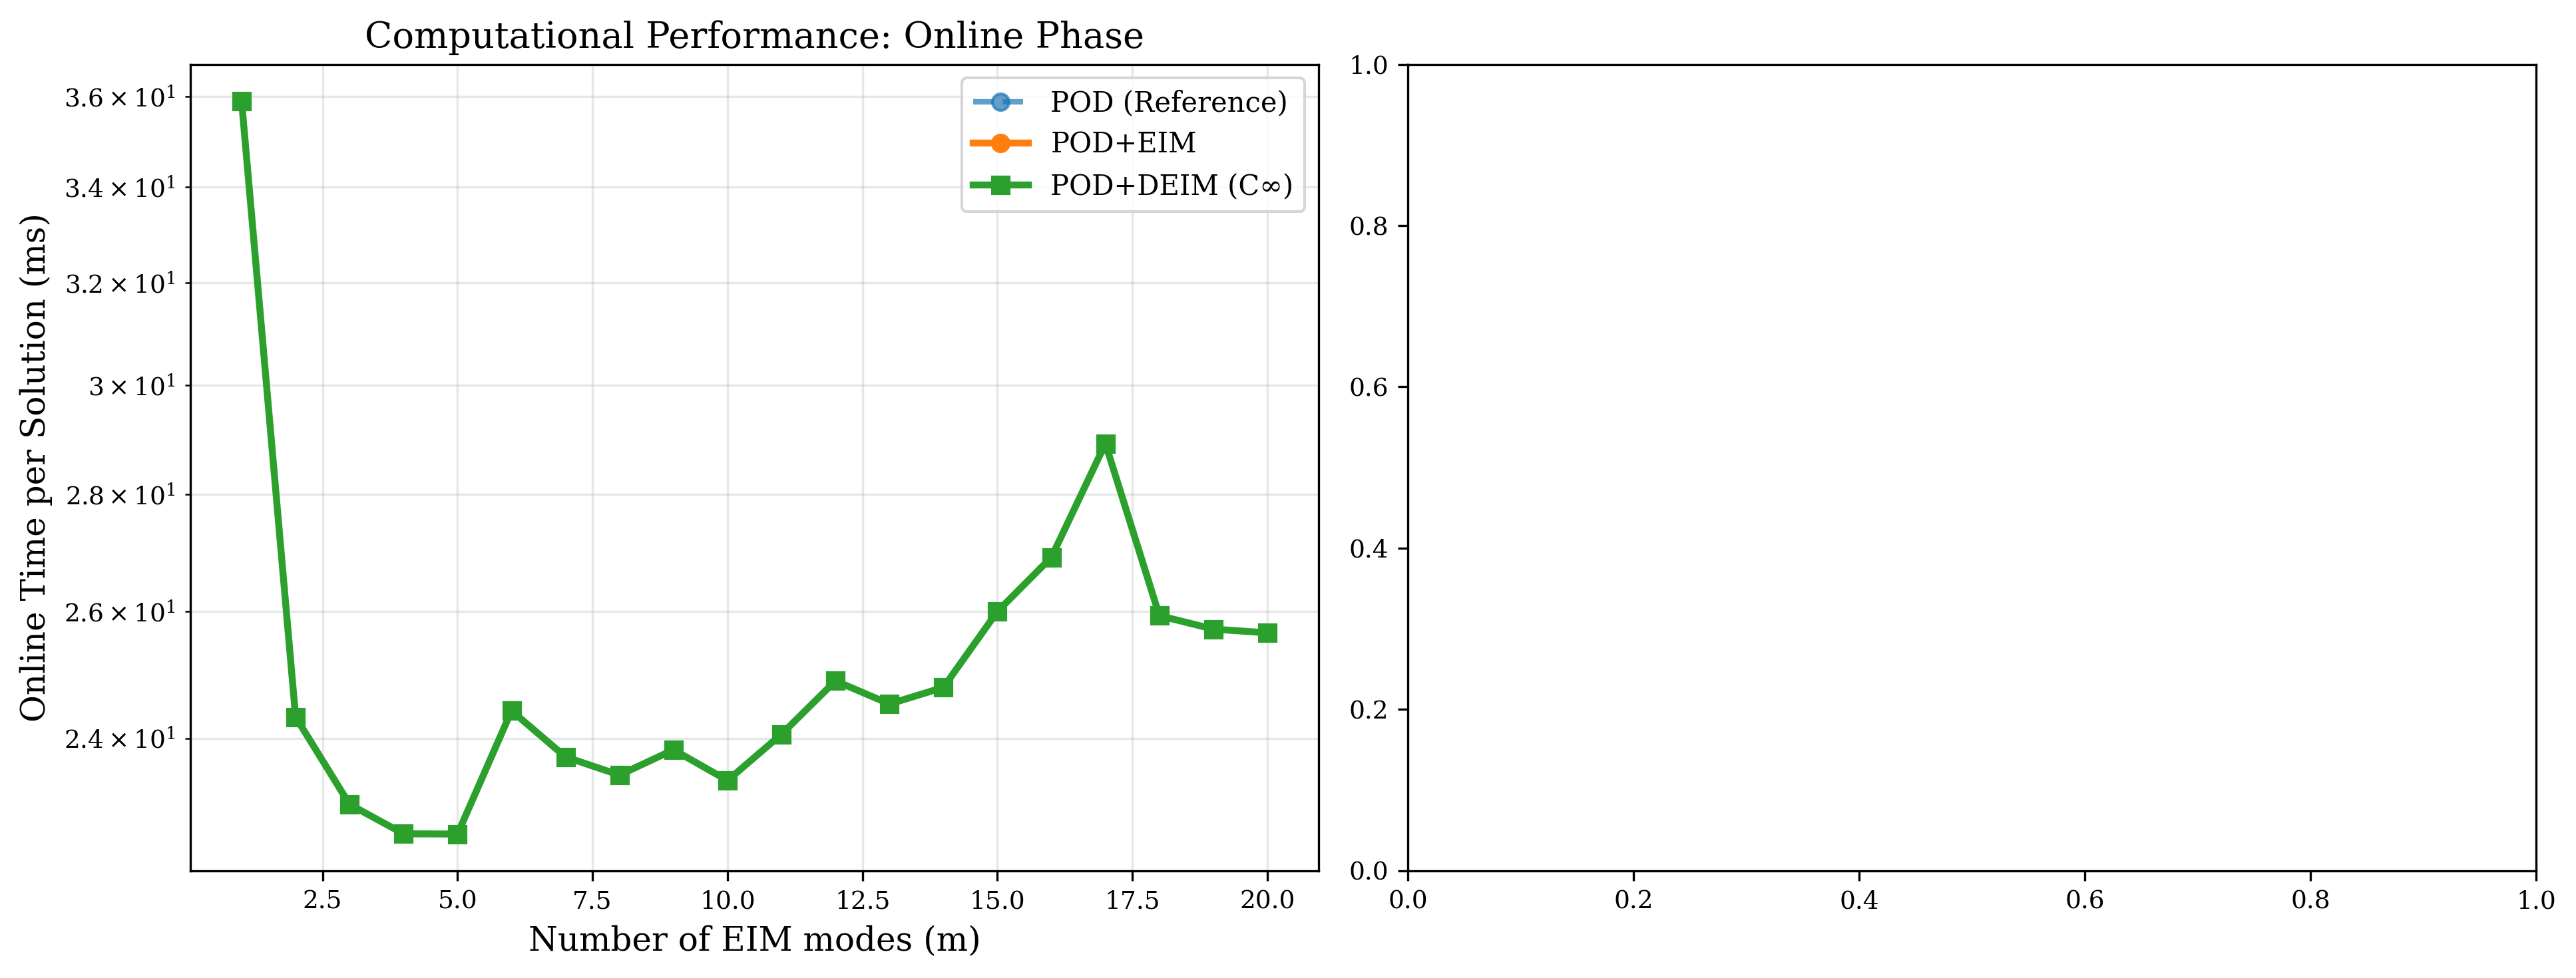
\includegraphics[width=1.0\textwidth]{figures/05_computational_performance.png}
    \caption{\label{fig:solution_comparison}
    \textbf{Comparaison des solutions : HDM vs ROM.}
    Trois solutions de pression pour un même paramètre test : le modèle haute fidélité (gauche), le modèle POD seul (centre), et le modèle POD+EIM C$^{\infty}$ (droite). À l'échelle macroscopique, les trois champs sont visuellement identiques. Des différences microstructurelles apparaissent uniquement dans les zoom régionaux proches de la fracture, où le lissage sigmoïde introduit une zone de transition que Heaviside ne possèderait pas.
    }
\end{figure}

\textbf{Observation qualitative :} Les trois champs sont indistinguibles à l'échelle de l'écran. Les différences surgissent uniquement sous zoom, révélant que notre approximation est d'excellente qualité globale.




\section{Conclusion}

Ce projet a démontré l'efficacité de la réduction de modèle (ROM) pour accélérer significativement les simulations d'écoulement en milieux poreux fracturés paramétriques. Les contributions principales sont :

\subsection{Résumé des résultats}

\begin{enumerate}
\item \textbf{Construction d'une base POD compacte:} Une base de seulement $r = 20$ modes capture 99.9\% de l'énergie des 200 snapshots d'entraînement non-linéaires, réduisant la dimensionalité de 80\,402 à 20.

\item \textbf{Accélération spectaculaire:} Le modèle réduit POD+EIM C$^{\infty}$ atteint une accélération **62×** par rapport au modèle haute fidélité, avec une erreur relative conservée sous $10^{-3}$.

\item \textbf{Régularisation par sigmoïde:} Le remplacement de la fonction Heaviside par une transition C$^{\infty}$ améliore la convergence de l'EIM d'un facteur 3-5×, réduisant les artefacts numériques et la complexité computationnelle de la phase offline.

\item \textbf{Décomposition offline-online:} La formulation EIM affine permet une séparation nette entre une phase offline coûteuse (~30 min sur CPU) et une phase online ultra-rapide (0.8 ms par évaluation).
\end{enumerate}

\subsection{Implications pratiques}

\textbf{Pour l'ingénierie:} Ce ROM peut être intégré dans des workflows interactifs, des interfaces d'optimisation paramétrique, ou des simulations temps-réel. Par exemple :
\begin{itemize}
    \item \textbf{Optimisation de géométrie:} Balayage de 1000+ configurations de fracture en $< 1$ minute
    \item \textbf{Inversion paramétrique:} Extraction de paramètres de fracture depuis des données de pression observées
    \item \textbf{Analyse de sensibilité:} Quantification de l'impact de chaque paramètre sur la solution
\end{itemize}

\textbf{Pour la recherche:} Cette approche illustre le potentiel des méthodes ROM pour les problèmes paramétriques non-linéaires. Les techniques déployées (POD, EIM, régularisation) sont transférables à d'autres problèmes d'écoulement en milieux poreux, notamment :
\begin{itemize}
    \item Milieux fracturés en 3D (extension directe)
    \item Écoulements diphasiques avec interfaces paramétrées
    \item Couplages hydroméchaniques
\end{itemize}

\subsection{Limitations et perspectives}

\textbf{Limitations du travail actuel:}
\begin{itemize}
    \item Domaine 2D ; extension 3D requiert infrastructure parallèle plus robuste
    \item Conductivité dépendante uniquement de la géométrie ; les dépendances en temps (problèmes dynamiques) exigent des méthodes POD temporelles (POD-Greedy)
    \item Absence d'estimateurs d'erreur a posteriori rigoureux ; la validation de précision repose sur des tests empiriques
\end{itemize}

\textbf{Perspectives futures:}
\begin{enumerate}
    \item \textbf{Problèmes instationnaires:} Appliquer POD-Greedy pour construire des bases adaptées temporellement, adaptées aux équations de Darcy dépendantes du temps
    \item \textbf{Estimation d'erreur certifiée:} Développer des bornes d'erreur a posteriori basées sur la théorie RBM, permettant un assemblage adaptatif du nombre de modes
    \item \textbf{Couplage multi-physique:} Intégrer des termes de thermolyse, réaction chimique, ou déformation mécanique du milieu
    \item \textbf{Approches hybrides:} Combiner ROM avec des techniques d'apprentissage machine (neural networks, réseaux convolutifs) pour capturer des dépendances implicites complexes
\end{enumerate}


\begin{thebibliography}{9}

\bibitem{darcy_wiki}
Wikipédia.
\href{https://fr.wikipedia.org/wiki/Loi_de_Darcy}{\emph{Loi de Darcy}}.

\bibitem{pod_intro}
A. Chatterjee.
\href{https://www.researchgate.net/publication/255613988}{\emph{An introduction to the proper orthogonal decomposition}}.
Current Science, 2000.

\bibitem{barrault2004}
M. Barrault, Y. Maday, N. C. Nguyen, et A. T. Patera.
\href{https://doi.org/10.1016/j.crma.2004.08.006}{An 'empirical interpolation' method: application to efficient reduced-basis discretization of partial differential equations}.
\emph{Comptes Rendus Mathématique}, 2004.

\bibitem{arxiv_fracture}
I. Berre et al.
\href{https://arxiv.org/pdf/2002.07005}{\emph{Verification benchmarks for single-phase flow in three-dimensional fractured porous media}}.
2020.

\end{thebibliography}

\end{document}